\section{Modelo usando el dataset VarQ}

Comenzamos nuestro trabajo analizando el dataset construido en la tesis de Santiago Moreno. Este dataset fue construido inicialmente con las variantes originales del sitio de \textit{VarQ}, que consistieron en aproximadamente 400 mutaciones correspondientes a 13 proteínas con 10 variables. Posteriormente en el mismo trabajo se aumentó la cantidad para llegar a las aproximadamente 18 mil variantes del dataset VarQ usando otras fuentes como Clinvar y Humsavar. Llamaremos a este dataset VarQ Completo. 

\subsection{Variables del dataset VarQ Completo}

A continuación damos una descripción detallada de las variables originales encontradas en el dataset. Presentamos un extracto del trabajo de Santiago Moreno en donde se describen dichas variables [\todo{TOMADO DE TESIS DE SANTI}]: 

\begin{itemize}
    \item Variación de Energía (ENE): En VarQ, las mutaciones son modeladas con el software FoldX, que construye un modelo a partir de una estructura dada y luego muta residuos específicos. Luego el software predice el impacto energético de la mutación en la estabilidad de la proteína o, en caso de tratarse de un complejo, en la estabilidad del mismo.
    \item SASA: Es el valor correspondiente a la superficie accesible por parte del solvente, de la cadena lateral del aminoácido. Este valor permite determinar si la cadena lateral se encuentra en la superficie o en el núcleo de la estructura.
    \item Porcentaje de SASA: El porcentaje que representa el SASA sobre el total. Es decir el porcentaje que representa el SASA en función de la estructura de la proteína.
    \item B-Factor (BF): o factor de temperatura, que corresponde a un aminoácido dentro de la proteína. Una mayor temperatura, indica que el aminoácido pertenece a una zona potencialmente de mayor movilidad.
    \item Switchability (SWI): Evalúa cuán propenso a generar un cambio de hélice alfa a hoja beta es un conjunto de aminoácidos.
    \item Aggregability (AGG): El software Tango evalúa cuán
    propenso es un aminoácido a generar agregación en una proteína desde un punto de vista estructural. La agregación es el proceso por el cual proteínas mal formadas
    adoptan una conformación que causa su polimerización en fibrillas agregadas y organizadas. Muchas enfermedades neurodegenerativas, como por ejemplo la Amiloidosis, están asociadas con la agregación proteica.
    \item Conservación (CONS): Se calcula en bits, siempre y cuando la mutación pueda ser mapeada a una posición en una familia PFam asignada. Cuando una posición tiene un alto valor en bits y la misma posición coincide con el aminoácido conservado en la secuencia de la proteína interpretamos que dicha posición está altamente conservada. La misma puede estar altamente conservada porque es importante estructuralmente o porque es importante para la actividad enzimática. Los residuos con alta conservación tendrán un impacto mayor sobre la función pues afectan aminoácidos de la familia.
    \item Sitio Activo (AS): Las posiciones de sitio activo son aquellas que se encuentran marcadas como unidas a ligandos en los archivos PDB o que pertenecen al mismo pocket que se encuentren conteniendo estos residuos nombrados o aquellos que pertenezcan al Catalytic Site Atlas.
    \item Interfaz 3DID: Determina si la posición sirve para una interfaz proteína-proteína según la base de datos de 3DID.
    \item Interfaz PDB: Determina si la posición sirve para una interfaz proteína-proteína según la base de datos de PDB.
\end{itemize}


\subsection{Limpieza del dataset VarQ Completo}

Para trabajar con este dataset decidimos verificar la etiqueta de cada una de las variantes, de manera de confirmar que su status siguiera vigente. Para esto recurrimos a las fuentes Clinvar y Humsavar. Realizamos un primer filtrado de estas tablas quedándonos con aquellas variables con un status confirmado: en el caso de Humsavar, aquellas que figuran con la expresión \textit{Polymorphism} y \textit{Disease}, mientras que en Clinvar nos quedamos con aquellas que figuraban como \textit{Benign} y \textit{Pathogenic}, eliminando aquellas con caracterización difusa, por ejemplo, ``factor de riesgo''. 

\begin{figure}[H]
    \centering
    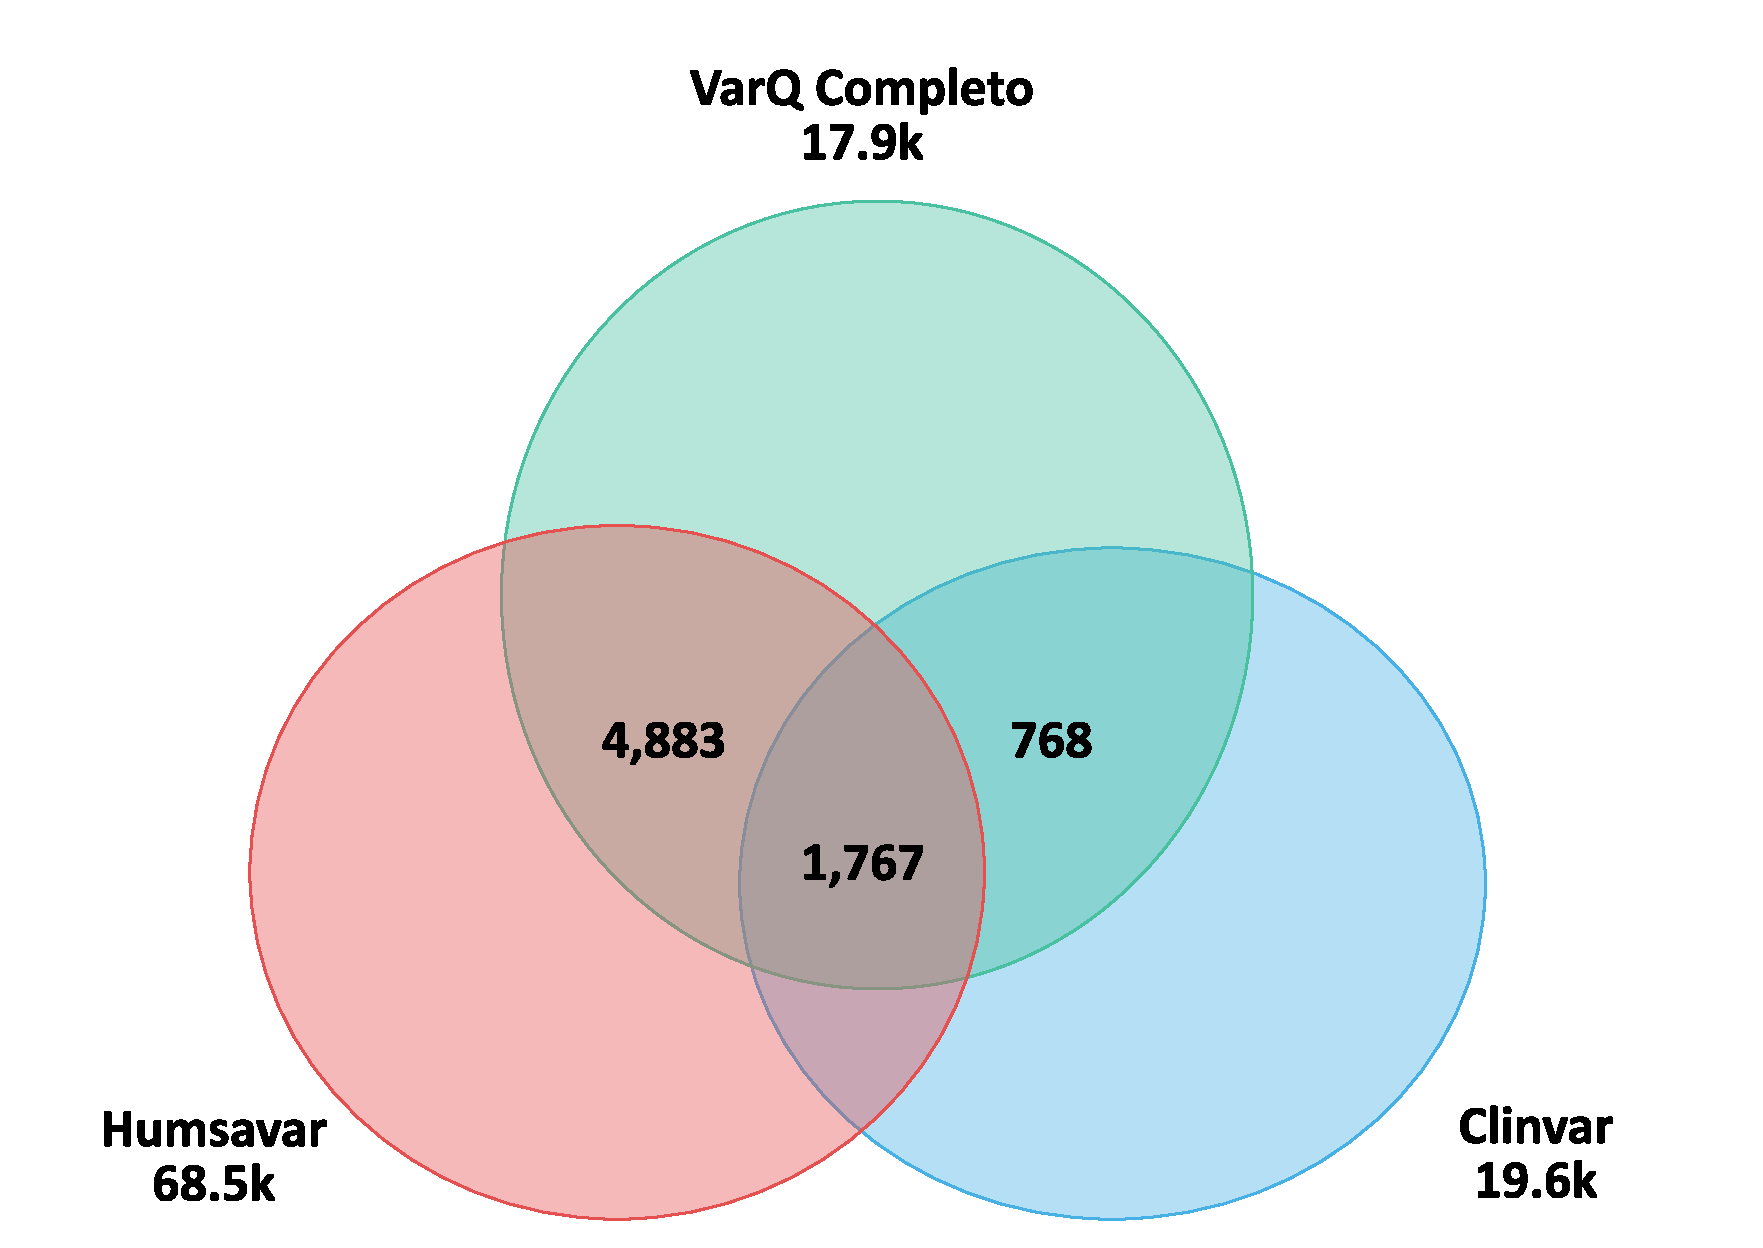
\includegraphics[scale=0.4]{documents/latex/figures/3/varq/interseccion_varq.pdf}
    \caption{Valores en la intersección del dataset VarQ Completo con las tablas Clinvar y Humsavar.}
    \label{fig:interseccion_varq}
\end{figure}

Así, cruzamos los datos con las tablas filtradas Humsavar y Clinvar, y encontramos un subconjunto importante de variantes que no aparecían en ninguna de las dos fuentes. Estas variantes estaban rotuladas en su gran mayoría (94\%) como benignas, por lo que creemos que se consideraron como variantes benignas a todas aquellas a las que no se encontró un reporte. Decidimos remover estas variantes del dataset por considerar que si alguna de ellas estuviera rotulada incorrectamente introduciría ruido. Como puede observarse en la figura \ref{fig:interseccion_varq}, de las 17,869 variantes del dataset VarQ Completo, logramos encontrar 2,535 en la tabla de Clinvar, de los cuales sólo 2,397 tenían un estado confirmado como patogénicas, y 138 como benignas. Cruzando el dataset con la tabla Humsavar encontramos una intersección de 6,650 variantes de los cuales 4,667 corresponden a patogénicas y 1,983 son benignas. Decidimos mantener la clasificación de Humsavar en la intersección de los tres conjuntos por considerarla de mayor confiabilidad dado que es un reporte único curado por expertos, a diferencia de Clinvar que es una recopilación de variantes de diversa significación clínica, y a menudo presenta conflictos de anotación por discrepancias entre evidencias reportadas. Esto nos deja con un dataset Curado de 7,418 variantes de las cuales 5,377 son patogénicas y 2,041 son benignas. Denominaremos a este dataset \textit{VarQ Curado}. 


\subsection{Descripción estadística del dataset VarQ Curado}

A partir de VarQ Curado estudiaremos sus variables usando estadísticas descriptivas con el objetivo de evaluar la calidad del dataset. La idea es poder tener una noción de la dispersión de nuestros datos, sumado a la cobertura que tenemos de ellos sobre las variantes. En la tabla \ref{tab:descripcion_varq_cont} podemos ver distintas métricas sobre las variables continuas del dataset, como la media de los valores (mean), el desvío estándar (std), el valor máximo (max) y los cuartiles. 

También sumamos a esta descripción el AUC univariado, es decir el área bajo la curva ROC tomando la variable ordenada como estimador de la respuesta.   

Un AUC cercano a 0.5 equivale a una variable de bajo poder predictivo, mientras que un AUC mayor a 0.5 corresponde a un predictor de la variable de respuesta (en este caso una variante patogénica), mientras que un AUC menor a 0.5 corresponde a un anti-predictor, es decir que invertir su respuesta equivale a un predictor de AUC mayor a 0.5. En la columna AUC de la tabla \ref{tab:descripcion_varq_cont} vemos que las variables SASA y SASA \% tienen un poder anti-predictivo relativamente alto (0.34 y 0.33 respectivamente), lo que indica que las variantes que tengan un valor elevado de estas variables tienden a ser benignas, mientras que la variación de energía tiene el mejor poder predictivo univariado entre todas las variables.

\begin{table}[H]
\centering
\begin{tabular}{|l|l|l|l|l|l|l|l|l|}
\hline
Variable & avg  & std   & min    & 25\%  & 50\%  & 75\%  & max & AUC\\ \hline
SASA    & 32.11 & 39.15 & 0.0    & 0.67  & 15.21 & 52.15 & 246.41 & 0.34 \\ \hline
SASA\%  & 0.15  & 0.18  & 0.0    & 0.0   & 0.07  & 0.27  & 0.75 & 0.33  \\ \hline
BFACTOR & 56.45 & 71.76 & 0.0    & 19.77 & 37.34 & 61.14 & 755.61 & 0.46 \\ \hline
SWITCH  & 0.38  & 0.89  & 0.0    & 0.0   & 0.01  & 0.28  & 8.72 &  0.50  \\ \hline
AGG     & 5.02  & 17.61 & 0.0    & 0.0   & 0.0   & 0.16  & 100.0 &  0.51\\ \hline
CONS    & 0.33  & 0.19  & 0.13   & 0.25  & 0.3   & 0.37  & 4.77 & 0.43\\ \hline
ENE     & 2.91  & 4.84  & -12.64 & 0.26  & 1.51  & 3.89 & 57.21 & 0.68\\ \hline 
\end{tabular}
\caption{Descripción de variables continuas del dataset \textit{VarQ Curado}.}
\label{tab:descripcion_varq_cont}
\end{table}

\begin{table}[H]
\centering
\begin{tabular}{|l|l|l|l|}
\hline
Variable & top  & freq. top & BACC \\ \hline
3DID & False & 0.8 & 0.51\\ \hline
PDB  & False  & 0.9 & 0.49\\ \hline
\end{tabular}
\caption{Descripción de variables categóricas del dataset \textit{VarQ Curado}.}
\label{tab:descripcion_varq_cat}
\end{table}

Para el caso de las variables categóricas (PDB y 3DID), analizamos el valor con la frecuencia más alta (top) y la frecuencia de este valor. Para este tipo de variables quisimos también cuantificar su poder predictivo individual. 

% \newpage

Utilizar AUC en este caso no es posible dado que su cálculo sólo tiene sentido en variables continuas. Por lo tanto, decidimos calcular el \textit{Balanced Accuracy} (BACC) \cite{Brodersen2010} como medida de poder predictivo, considerando el valor de la variable como predictor de la variante. 

El \textit{Balanced Accuracy} (BACC) es igual a:
\begin{equation*}
    \frac{1}{2} (\frac{VP}{P} + \frac{VN}{N})
\end{equation*}

Donde VP es igual a la cantidad de verdaderos positivos, P es igual a la cantidad de ejemplos etiquetados como positivos, VN es la cantidad de verdaderos negativos y N la cantidad de ejemplos etiquetados como negativos.

En la tabla \ref{tab:descripcion_varq_cat} podemos ver que el BACC de las variables 3DID y PDB es de 0.51 y 0.49 respectivamente, lo que indica un bajo valor predictivo. 

Otro de los puntos importantes durante la exploración del dataset es la detección de variables con muy poca cobertura. En la figura \ref{fig:proporcion_nulos_varq} podemos observar como la variable de sitio activo (ACTIVE\_SITE) no posee datos para casi ninguna variante (aproximadamente el 95\%), mientras que la variable de conservación (CONS) no posee datos para el 63\% de las variantes. En base a estas observaciones decidimos remover la variable de sitio activo del dataset por considerarla muy poco relevante en términos de cobertura.

\begin{figure}[H]
    \centering
    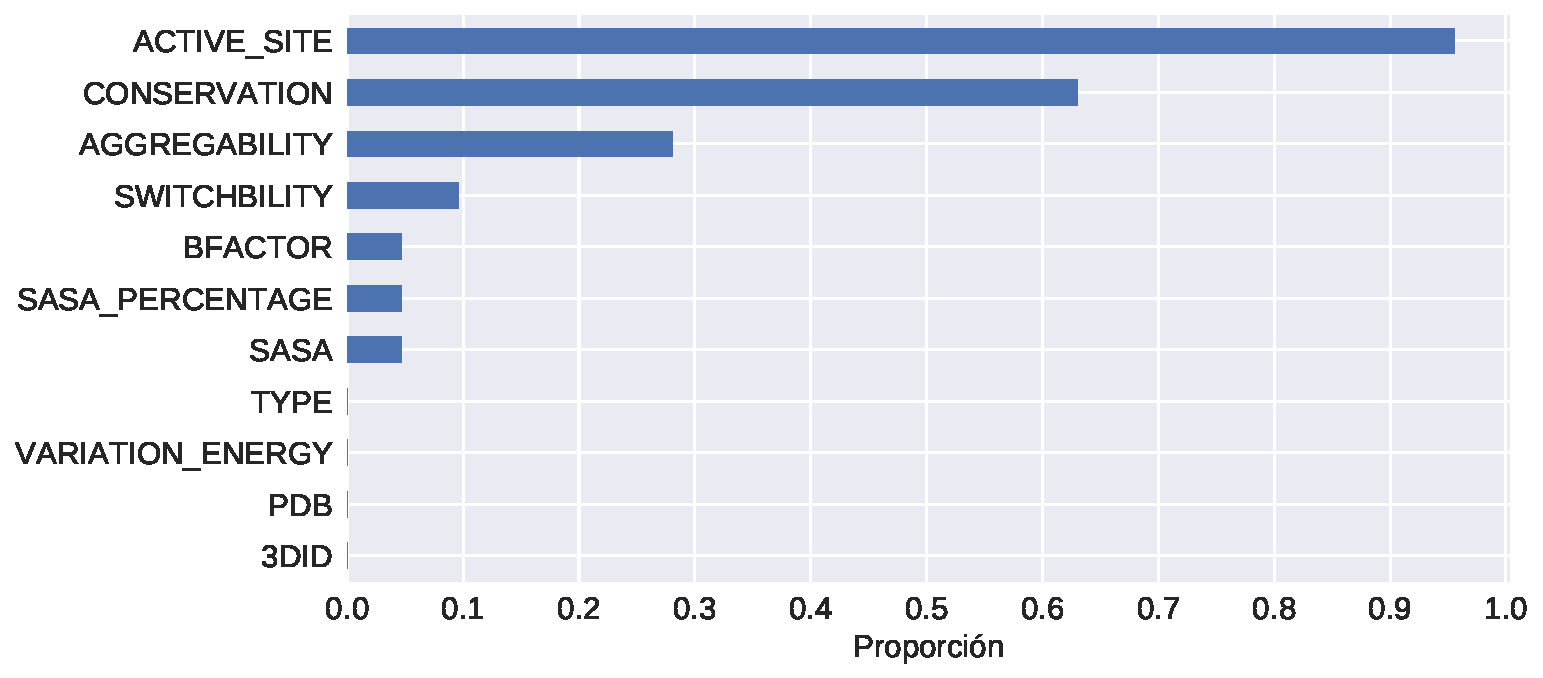
\includegraphics[scale=0.55]{documents/latex/figures/3/varq/proporcion_nulos.pdf}
    \caption{Proporción de variantes con valor nulo por variable del dataset VarQ Curado.}
    \label{fig:proporcion_nulos_varq}
\end{figure}

Otro factor importante a considerar es cuántas variables nulas tienen cada una de las variantes del dataset. En la figura \ref{fig:nulos_varq} podemos observar que existe aproximadamente un 5 \% de variantes que poseen 7 variables nulas de las 10 que contienen el dataset, es decir, prácticamente no tienen ningún tipo de información, y sólo el 2\% de las variantes posee el total de las variables cubiertas. Por el otro lado, casi el 90\% de las variantes tiene a lo sumo 3 variables nulas.

\begin{figure}[H]
    \centering
    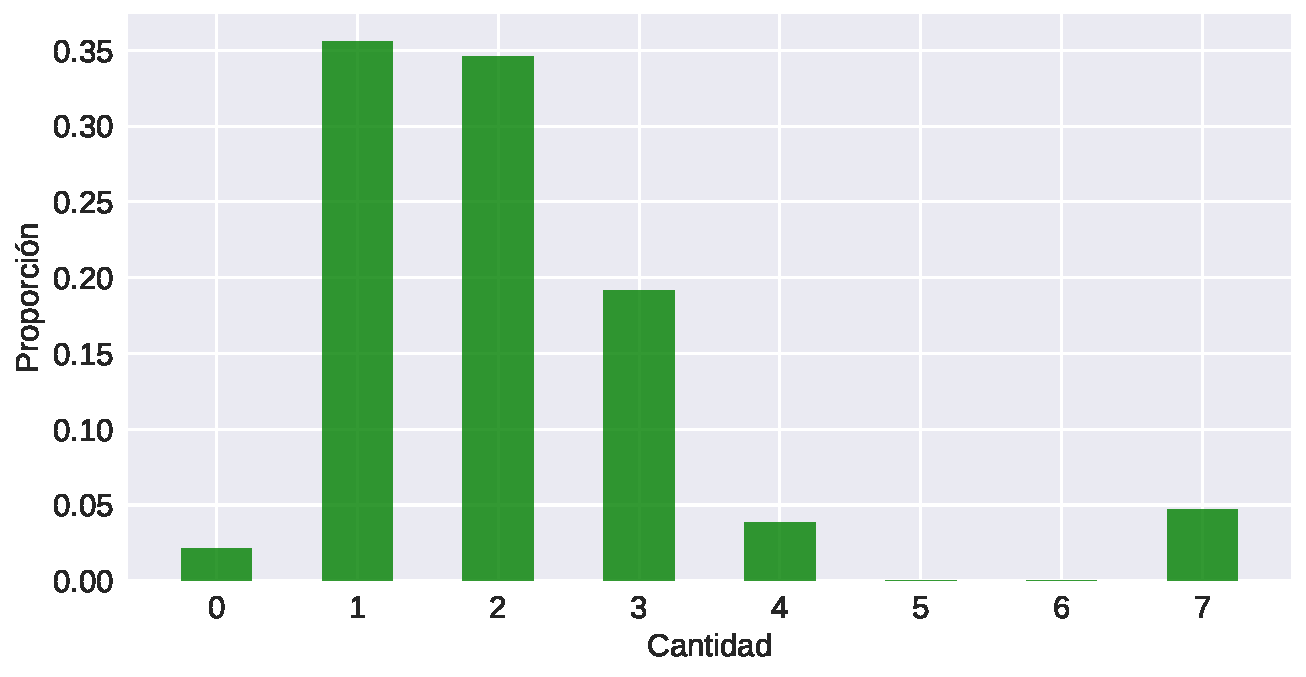
\includegraphics[scale=0.55]{documents/latex/figures/3/varq/nulos_varq.pdf}
    \caption{Histograma de cantidad de variables nulas del dataset VarQ Curado.}
    \label{fig:nulos_varq}
\end{figure}

\subsubsection{Correlación entre las variables de VarQ Curado}

También queremos conocer qué tan correlacionadas se encuentras las variables. En la figura \ref{fig:varq_corrplot} vemos la correlación de Spearman que sirve para detectar relaciones monotónicas entre las variables, y así nos permite descartar variables muy similares que no aportan nueva información y ralentizan el entrenamiento del modelo. De esta forma encontramos que la variable SASA y SASA\_PERCENTAGE tienen una correlación de 0.98.

\begin{figure}[H]
    \centering
    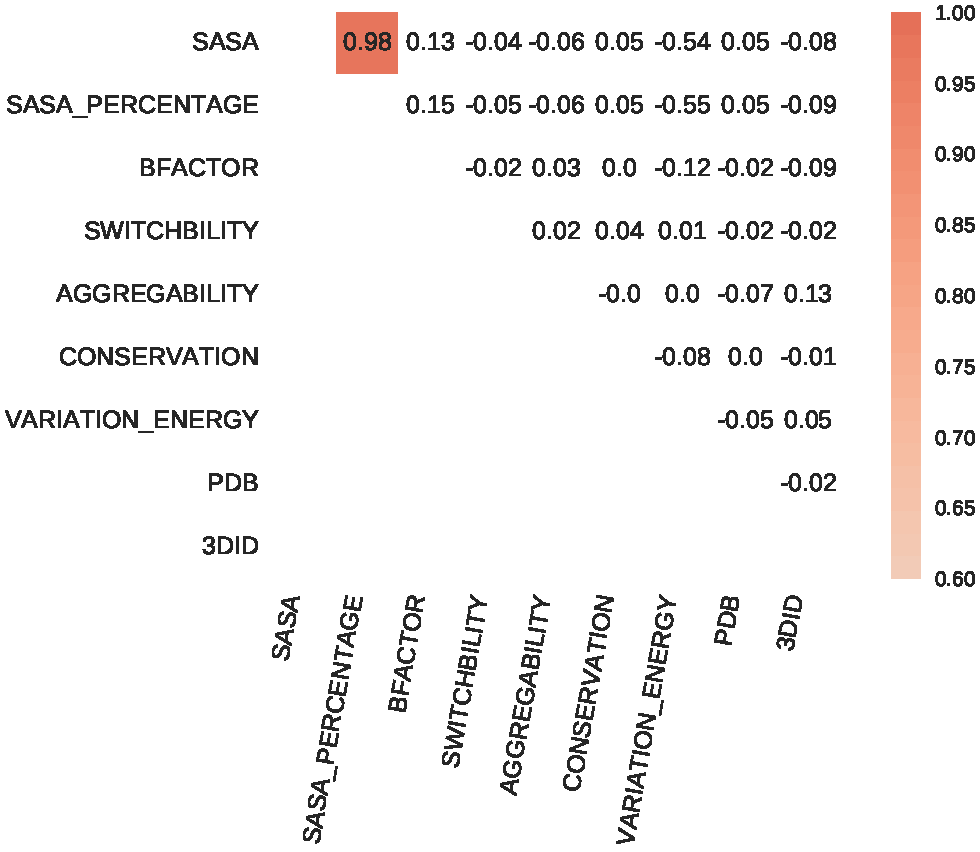
\includegraphics[scale=0.6]{documents/latex/figures/3/varq/varq_corrplot.pdf}
    \caption{Correlación de Spearman para las variables de VarQ Curado.}
    \label{fig:varq_corrplot}
\end{figure}

% \newpage

\subsection{Modelo creado a partir del dataset VarQ Curado}

Una vez definido el dataset, podemos emplear técnicas de aprendizaje automático con el objetivo de generar un predictor de variantes patogénicas. Cabe destacar, que en este dataset VarQ Curado hay una sobrerrepresentación de variantes patogénicas, es decir, que presenta un desbalance (mayor número de variantes patogénicas que benignas) que invierte las propociones observadas en el dataset VarQ Completo. De todas formas generaremos un modelo para poder evaluar de forma preliminar la dificultad del problema. 

Para esto recurrimos a diferentes algoritmos de aprendizaje automático: Support Vector Classifier (SVC), Regresión Logística y Random Forest. La construcción del pipeline para cada uno de estos algoEritmos constó de tres fases: 

\begin{itemize}
    \item \textbf{Creación del set de entrenamiento y de evaluación}: División (\textit{split}) estratificado (es decir, manteniendo las proporciones originales de la variable objetivoE) del dataset, 66\% para entrenamiento y 33\% para evaluación. 
    \item \textbf{Imputación de las variables}: Se reemplazaron los valores nulos de cada variable por su mediana en caso de las continuas y por el valor más frecuente en el caso de las variables categóricas.
    \item \textbf{Estandarización}: Para el caso de los algoritmos paramétricos (Regresión Logística y SVM) se aplicó una estandarización robusta a outliers. Esta estandarización consiste en restar la mediana del valor y escalar los datos de acuerdo a la distancia intercuartil, como se observa en la ecuación \ref{eq:robust_scaler}.
    
    \begin{equation}
        RobustScaling(x_i) = \frac{x_i - Q_2(\textbf{x})}{Q_3(\textbf{x}) - Q_1(\textbf{x})} 
        \label{eq:robust_scaler}
    \end{equation}
    
    donde $x_i$ corresponde al valor de la variable,  $Q_1$, $Q_2$ y $Q_3$ corresponde al primer, segundo y tercer cuartil de la variable $\textbf{x}$ respectivamente.
    
    
\end{itemize}

Luego del preprocesamiento, para cada uno de los algoritmos se realizó una búsqueda de hiperparámetros óptimos, a partir de estos datos, con la función \texttt{GridSearchCV} de la biblioteca \textit{Scikit-learn}. El objetivo de esta función es evaluar todas las combinaciones de hiperparámetros definidos en un diccionario y retornar el estimador que dio mejores resultados (de acuerdo a una métrica escogida, en este caso el área bajo la curva ROC). Esta métrica a su vez es evaluada a través de validación cruzada (\textit{3-fold Cross Validation}). En el apéndice se encuentran los diccionarios de hiperparámetros usados en cada uno de los modelos.

\subsection{Resultados}

Random Forest fue el mejor modelo con un AUC de 0.74. Los parámetros óptimos de este modelo fueron una profundidad de árbol de 7, 100 estimadores y una cantidad máxima de variables por árbol de 4.

La Regresión logística y SVC obtuvieron 0.71 y 0.70 respectivamente. Estos modelos se caracterizaron ademas por tener una tendencia a clasificar a las variantes como patogénicas, lo que se puede observar en su alto recall y menor precisión con respecto a Random Forest. En particular, SVC clasificó a todas las variantes del dataset de evaluación como patogénicas.

\begin{table}[H]
\centering
\begin{tabular}{|l|l|l|l|l|l|l|l|}
\hline
Modelo & Precisión & Recall & AUC & F1-score & F2-score & $t_{fit}$ & $t_{pred}$ \\ \hline
SVC    & 0.72 & \textbf{1.00} & 0.70 & 0.84 & \textbf{0.93} & 2 m 39 s & 0.77s \\ \hline
LR     & 0.75 & 0.94 & 0.71 & 0.84 & 0.90 & \textbf{1.17 s} & \textbf{0.01 s} \\ \hline
RF     & \textbf{0.77} & 0.93 & \textbf{0.74} & 0.84 & 0.89 & 9.82 s & 0.11 s \\ \hline
\end{tabular}
\label{tab:metrics_model}
\end{table}




La tabla \ref{tab:metrics_varq} muestra algunas métricas de interés obtenidas del modelo Random Forest para entender mejor los resultados del modelo basados en el predictor generado.



\begin{table}[H]
\centering
\begin{tabular}{|l|l|l|l|}
\hline
              & Precisión & Recall & F1-score \\ \hline
Benignas      & 0.57      & 0.26   & 0.36     \\ \hline
Patogénicas   & 0.77      & 0.93   & 0.84     \\ \hline
Promedio      & 0.71      & 0.74   & 0.71     \\ \hline
\end{tabular}
\caption{Reporte de métricas del modelo Random Forest usando el dataset VarQ Curado.}
\label{tab:metrics_varq}
\end{table}

La precisión del modelo indica un número marcadamente bajo (0.57) en la clase benigna, lo que significa que casi una de cada dos variantes detectadas como benignas es en efecto patogénica. El Recall con respecto a las variantes benignas es de 0.26, es decir que el modelo sólo reconoce alrededor de un cuarto de las variantes benignas como tales. Por lo tanto podemos afirmar que este modelo tiene una tendencia a calificar las variantes como patogénicas, generando una gran cantidad de falsos positivos (o Error de tipo I). Es importante remarcar que estas métricas están generadas a partir de una función de decisión o \textit{threshold} fijado por la versión del algoritmo usado (en el caso de la librería \texttt{scikit-learn}, este \textit{threshold} está ubicado en 0.5 de la probabilidad asignada).  La curva ROC, o \textit{Receiver Operating Characteristic} y su AUC asociada, nos permite independizarnos de un \textit{threshold} fijo para evaluar las características del predictor (fig 1.5a).

En la figura \ref{fig:importance_varq} podemos observar la importancia de los features reportado por el algoritmo Random Forest, que ubica en primer lugar con una gran diferencia a la variable que hace referencia a la Variación de Energía (ENE), seguido por el BFACTOR y el porcentaje de SASA (SASA \%). Este dato concuerda parcialmente con sus valores de AUC univariado. Si bien ENE y SASA \% poseen un valor relativamente alto de poder de clasificación univariada, no sucedía lo mismo con BFACTOR. En el modelo multivariado esta situación se invierte.

\newpage

\begin{figure}[H]
\centering
\begin{subfigure}{0.7\textwidth}
    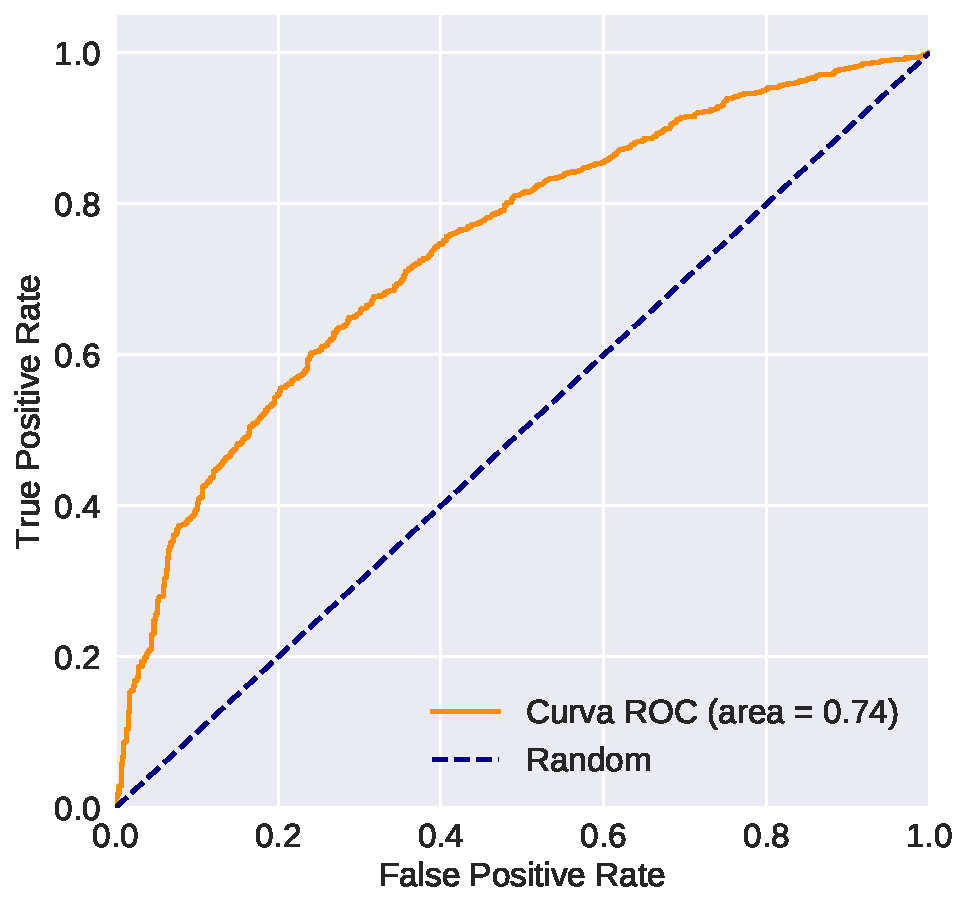
\includegraphics[width=\textwidth]{documents/latex/figures/3/varq/auc_varq.pdf}
    \caption{Curva ROC del algoritmo Random Forest del dataset VarQ Curado. La línea punteada corresponde a la curva ROC de un estimador aleatorio, o \textit{Random}, cuyo AUC es igual a 0.5.}
    \label{fig:auc_varq}
\end{subfigure}
\begin{subfigure}{0.7\textwidth}
    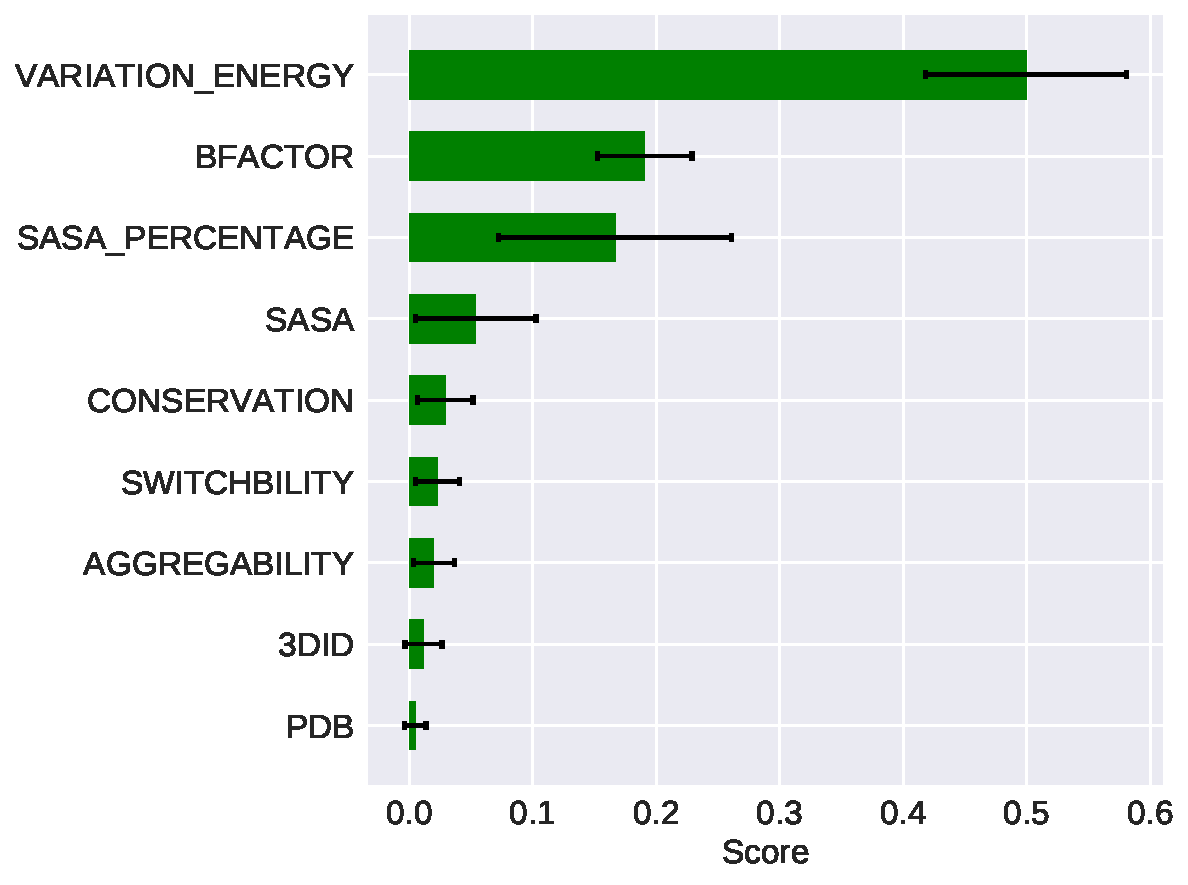
\includegraphics[width=\textwidth]{documents/latex/figures/3/varq/importances_varq.pdf}
    \caption{Los atributos del dataset VarQ Curado en orden de importancia usando un modelo Random Forest. La barra de error corresponde al desvío estándar del \textit{Feature Importance} de cada uno de los árboles del modelo.}
    \label{fig:importance_varq}
\end{subfigure}
\end{figure}

% \newpage

\section{Modelo usando propiedades físico-químicas de la proteína}

En esta sección generamos un nuevo dataset buscando nuevas fuentes de información de carácter físico-químico de las proteínas. Estas variables provienen de dos fuentes principales:

\begin{itemize}
    \item El módulo ProtParam proveniente de la biblioteca Biopython \cite{Chapman:2000:BPT:360262.360268}
    \item La base de datos SNVBox del laboratorio Karchin \cite{Wong2011}
\end{itemize}

Para el análisis de estas variables usamos la tabla Humsavar. La tabla Humsavar (a Noviembre 2017) está compuesta originalmente por 75,769 variantes (o ``mutantes'') de las cuales 39,653 son benignas (52\%), 28,855 (38\%) están asociadas a enfermedades y 7,261 (10\%) no están clasificadas. Las variantes no clasificadas fueron descartadas. 

\subsection{Extracción de variables usando Biopython}

La primera fuente que utilizamos, por su relativa practicidad de uso en la extracción de un conjunto de variables físico-químicas de la proteína, fue el módulo ProtParam de la biblioteca Biopython. Esta biblioteca es un set de herramientas escritas en Python, desarrollada por un equipo internacional de desarrolladores para el área de la bioinformática, y posee una licencia de uso libre.
El nombre ProtParam proviene de \textit{Protein Parameters} (parámetros de la proteína) y está basado en la herramienta homónima del server proteómico Expasy. Para ser utilizado el módulo requiere el \textit{accession number} de la proteína (identificador único) o una subsecuencia de la misma, para poder acceder a los parámetros calculados, que son los siguientes:

\begin{itemize}
    \item Punto isoeléctrico teórico (ISO\_POINT): pH en el que la proteína (o subsecuencia) tiene carga nula. 
    \item Aromaticidad (AROM): La frecuencia relativa de la subsecuencia Phe+Trp+Tyr (Fenilalanina, Triptófano y Tirosina). 
    \item Índice de inestabilidad (INST): Testea la estabilidad de la subsecuencia. Cualquier valor superior a 40 indica inestabilidad, es decir una corta semivida.
    \item Flexibilidad (FLEX): Método de Flexibilidad implementado por Vihinen et Al.  
    \item Promedio de hidrofobicidad (GRAVY): La suma de valores de hidrofobicidad de cada uno de los aminoácidos que componen la subsecuencia de la proteína.
\end{itemize}

Para poder utilizar el módulo ProtParam recurrimos a Uniprot con el fin de conseguir el proteoma humano en formato FASTA. El formato FASTA fue desarrollado por David Lipman y William Pearson en 1985, y originalmente fue incluido en un programa del mismo nombre utilizado para el alineamiento múltiple de secuencias. Una archivo FASTA puede incluir diferentes secuencias, no necesariamente de aminoácidos, y cada una de estas secuencias posee una línea de descripción al comienzo que empieza con el símbolo $>$. Por ejemplo, así se ve la secuencia de la Ovoalbúmina, una proteína de la especie Gallus gallus (gallina), o en otras palabras, la principal proteína que encontramos en la clara de los huevos (figura \ref{code:fasta_code})

\begin{figure}
% \centering
    \begin{verbatim}
    	>P01013 GENE X PROTEIN (OVALBUMIN-RELATED)
    	QIKDLLVSSSTDLDTTLVLVNAIYFKGMWKTAFNAEDTREMPFHVTKQESKPVQMMCMNNSFNVATLPAE
    	KMKILELPFASGDLSMLVLLPDEVSDLERIEKTINFEKLTEWTNPNTMEKRRVKVYLPQMKIEEKYNLTS
    	VLMALGMTDLFIPSANLTGISSAESLKISQAVHGAFMELSEDGIEMAGSTGVIEDIKHSPESEQFRADHP
    	FLFLIKHNPTNTIVYFGRYWSP
    \end{verbatim}
% \includegraphics{}
\caption{Ejemplo de código Fasta. Este código representa la proteína albúmina, donde cada letra representa un aminoácido, por ejemplo, las primeras 5 letras representan Q (glutamina), I (isoleucina), K (lisina), D (ácido aspártico) y L (leucina).}
\label{code:fasta_code}

\end{figure}
\pagebreak

A partir del proteoma obtenido se extrajeron las secuencias correspondientes a las proteínas del dataset Humsavar, y para cada una de ellas se tomó una subsecuencia de la misma de largo 7, alrededor de la posición donde se produjo la variante (figura \ref{fig:sequence_window}). En caso de que la variante se haya producido en los primeros o los últimos lugares, se toman aminoácidos a derecha o a izquierda según corresponda para completar el largo de la ventana.

% \begin{figure}
% \begin{textopo}
%   \labelstyle{hl}{diamond}{Black}{Blue}{White}{}
%   \sequence{PQALPSV[LQIAMAFGLAIGTLVQALG]HV%
%   SGAH[([NNE,30]hl[box[Black,Blue]:Half loop[White]]=INPAVTVACL)]VGCHVSFLR}
%   \Nterm{extra} \hideNterm \hideCterm \hidelegend \labelTM{1}{II}
%   \labeloutside[right]{extra}
% \end{textopo}
% \caption{A `half loop' example}\label{fighalf}
% \end{figure}

\begin{figure}[H]
    \centering
    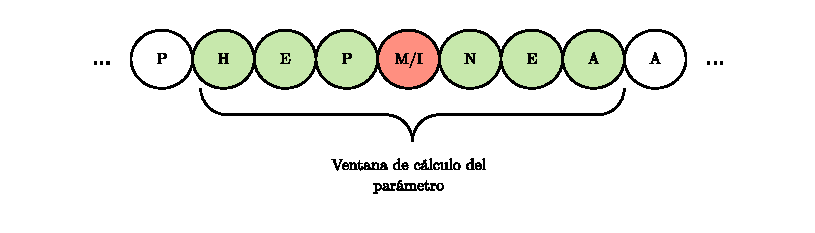
\includegraphics[scale=1.2]{documents/latex/figures/3/structural/protparam.pdf}
    \caption{Secuencia de aminoácidos de la proteína Arilacetamida deacetilasa (Q5VUY0). La ventana de la subsecuencia está marcada en verde, y la posición rojo es la mutación estudiada. En este caso la metionina (M) en la posición 307 fue reemplazada por una isoleucina (I).}
    \label{fig:sequence_window}
\end{figure}

A partir de los parámetros parámetros calculados en ProtParam, buscamos capturar la magnitud del cambio debido a la variante. Estos cambios pueden ser responsables de un efecto patogénico. Por ejemplo, si la región afectada por la variante pasa a ser hidrofílica en vez de hidrofóbica esta será más propensa a efectos adversos \cite{doi:10.1093/bioinformatics/btt308}.

En este sentido, generamos dos variables que buscan reflejar la diferencia generada por la variante. Las variables son las siguientes: 

\begin{itemize}
    \item Diferencia (DIFF) 
    $$|x - x_{var}|$$
    \item Cociente de logaritmos (LOG\_RATIO)
    $$\frac{\log{(x + 1)}}{\log{(x_{var} + 1)}}$$  
\end{itemize}

donde $x$ representa al parámetro original y $x_{var}$ es igual al parámetro de la variante.

\subsection{Extracción de variables usando SNVBox}

Además de la información obtenida vía ProtParam, recurrimos a una base de datos llamada SNVBox. Esta base de datos fue elaborada y es actualmente mantenida por el Karchin Lab de la Universidad Johns Hopkins. Se encuentra en su versión 3.0 y sigue en desarrollo. SNVBox posee alrededor de 90 variables consideradas relevantes para detectar el impacto biológico de un SNV (\textit{Single Nucleotide Variant}). Existen distintos criterios para definir un SNV y su diferencia de un SNP, pero en este trabajo los usaremos de forma indistinta. SNVBox posee datos físico-químicos de la proteína, a nivel de aminoácido y también a nivel de los sitios de la proteína donde se encuentra la variante. Otra característica destacable de esta fuente es que posee dichas variables para todos los codones del exoma humano.

\subsection{Generación del dataset Físico-Químico}

Luego del proceso del extracción de variables de Biopython y SNVBox, generamos un nuevo dataset cruzando sus atributos con las variantes de Humsavar. En el caso de los atributos relativos a los aminoácidos, pudimos cruzarlos usando la columna del dataset referente al identificador de la proteína, la posición de la variante, y el par de aminoácidos que se intercambiaron. Una vez agregadas todas las variantes a la tabla Humsavar, removimos todas aquellas variantes sin clasificación (etiqueta \textit{Unclassified}). El dataset resultante (denominado dataset Físico-Químico) está compuesto por 68,508 observaciones y 50 variables, incluyendo la variable de respuesta (o tipo), de las cuales 39,653 son benignas (no se encontraron reportes de enfermedades en la literatura), y 28,855 variantes están asociadas a alguna enfermedad. 

\subsection{Descripción estadística del dataset Físico-Químico}

Luego de la creación del dataset realizamos una exploración estadística del mismo, tal como hicimos en el dataset VarQ Curado. Calculamos la media (\textit{mean}), el desvío estándar (\textit{std}), el mínimo y los cuartiles (25\%, 50\%, y 75\%). También calculamos el AUC univariado para cada una de las variables continuas del dataset. Con respecto al AUC univariado en las variables de Protparam (tabla \ref{tab:protparam_vars}), notamos que la versión DIFF de los parámetros es mejor (anti) predictor que sus versiones LOG\_RATIO en todos los casos.


\begin{table}[H]
\centering
\begin{tabular}{|l|l|l|l|l|l|l|l|}
\hline
Variable & mean & std & min & 25\% & 50\%  & 75\%  & AUC \\ \hline
AROM\_DIFF  & 0.02  & 0.02  & 0.00 & 0.00 & 0.00  & 0.01  & 0.59 \\ \hline
AROM\_LOG\_RATIO & 1.97 & 0.33 & 1.00 & 1.94 & 1.94  & 1.94  & 0.53 \\ \hline
ISO\_POINT\_DIFF & 0.69  & 0.98 & 0.00  & 0.00 & 0.17  & 1.22  & 0.56 \\ \hline
ISO\_POINT\_LOG\_RATIO & 2.00 & 0.08 & 1.69 & 1.99 & 2.00  & 2.01  & 0.51 \\ \hline
GRAVY\_DIFF & 0.23 & 0.17 & 0.00 & 0.09 & 0.20  & 0.33  & 0.55 \\ \hline
GRAVY\_LOG\_RATIO & 1.99x10$^{12}$ & 1.24x$10^{14}$ & -3.39x10$^{15}$ & 1.43 & 1.94 & 2.43 & 0.48 \\\hline
INST\_DIFF & 14.02 & 13.27 & 0.00 & 4.20 & 10.09 & 20.10 & 0.49 \\ \hline
INST\_LOG\_RATIO & 2.06 & 2.27 & -84.77 & 1.96 & 2.01  & 2.09  & 0.48 \\ \hline
FLEX\_DIFF & 0.01 & 0.01 & 0.00 & 0.00 & 0.01  & 0.01  & 0.54 \\ \hline
FLEX\_LOG\_RATIO & 2.00 & 0.01 & 1.97 & 1.99 & 2.00  & 2.01  & 0.47 \\ \hline
\end{tabular}
\caption{Variables extraídas de Protparam}
\label{tab:protparam_vars}
\end{table}

\newpage

Con respecto al AUC univariado de las variables extraídas de SNVBox, notamos que las mejores variables en este respecto son las aportadas por algunas de las matrices de sustitución (EX, PAM250 y BLOSUM). En este caso son buenos anti-predictores, lo que indica que un valor bajo en esta matrix aporta una mayor probabilidad de ser patogénica (tabla \ref{tab:snvbox_amino}). El mejor predictor en este set de variables es la valor en la matriz de distancias GRANTHAM.  

% \newpage

% \subsubsection{Variables extraídas de SNVBox relativas a sustitución de aminoácidos}

\begin{table}[H]
\centering
\begin{tabular}{|l|l|l|l|l|l|l|l|}
\hline
Variable & mean   & std    & min    & 25\%  & 50\%   & 75\%   & AUC    \\ \hline
CHARGE            & 0.00  & 0.71   & -2.00  & 0.00  & 0.00   & 0.00   & 0.50   \\ \hline
VOLUME            & -0.16  & 1.70   & -5.59  & -1.40 & -0.16  & 0.96   & 0.48   \\ \hline
HYDROPHOBICITY    & -0.63  & 6.81   & -15.70 & -3.10 & -0.40  & 1.90   & 0.52  \\ \hline
GRANTHAM          & 79.96  & 48.06  & 5.00   & 43.00 & 74.00  & 102.00 & \textbf{0.63} \\ \hline
POLARITY          & -0.25  & 2.72   & -8.10  & -2.20 & -0.10  & 1.10   & 0.52   \\ \hline
EX                & 28.99  & 10.95  & -1.00  & 21.00 & 29.00  & 35.00  & \textbf{0.35}  \\ \hline
PAM250            & 0.16   & 1.68   & -5.40  & -1.00 & 0.20   & 1.40   & \textbf{0.36}   \\ \hline
BLOSUM            & -0.58  & 1.65   & -4.00  & -2.00 & -1.00  & 1.00   & \textbf{0.35}   \\ \hline
JM                & 0.80   & 1.24   & -1.73  & -0.50 & 1.05   & 1.66   & 0.40   \\ \hline
VB                & 19.78  & 14.64  & 0.00   & 8.00  & 17.00  & 29.00  & 0.42  \\ \hline
TRANSITION        & 0.00   & 0.00   & 0.00   & 0.00  & 0.00   & 0.00   & 0.47   \\ \hline
\end{tabular}
\caption{Variables extraídas de SNVBox relativas a sustitución de aminoácidos.}
\label{tab:snvbox_amino}

\end{table}

Describimos 21 variables de nuestro dataset. Las 29 variables restantes son extraídas de SNVBox relativas a proteínas y son todas categóricas de tipo \textit{Boolean} por lo que destacamos algunos datos de relevancia (ver apéndice para un listado completo). Todas estas variables tienen una cobertura para aproximadamente el 31.5\% de las variantes del dataset, y cada una de ellas poseen valor Falso para un porcentaje superior al 90\% de las variantes de la tabla, exceptuando las variables \textbf{TRANSMEM} (82\%), \textbf{REP} (87\%), \textbf{REGIONS} (70\%) y \textbf{PPI} (87\%). El \textit{Balanced Accuracy} de estas variables oscilan entre el 0.45 y 0.48, lo que connota un bajo poder predictivo univariado.


\newpage
% \subsubsection{Correlación entre las variables}

\begin{figure}[H]
    \centering
    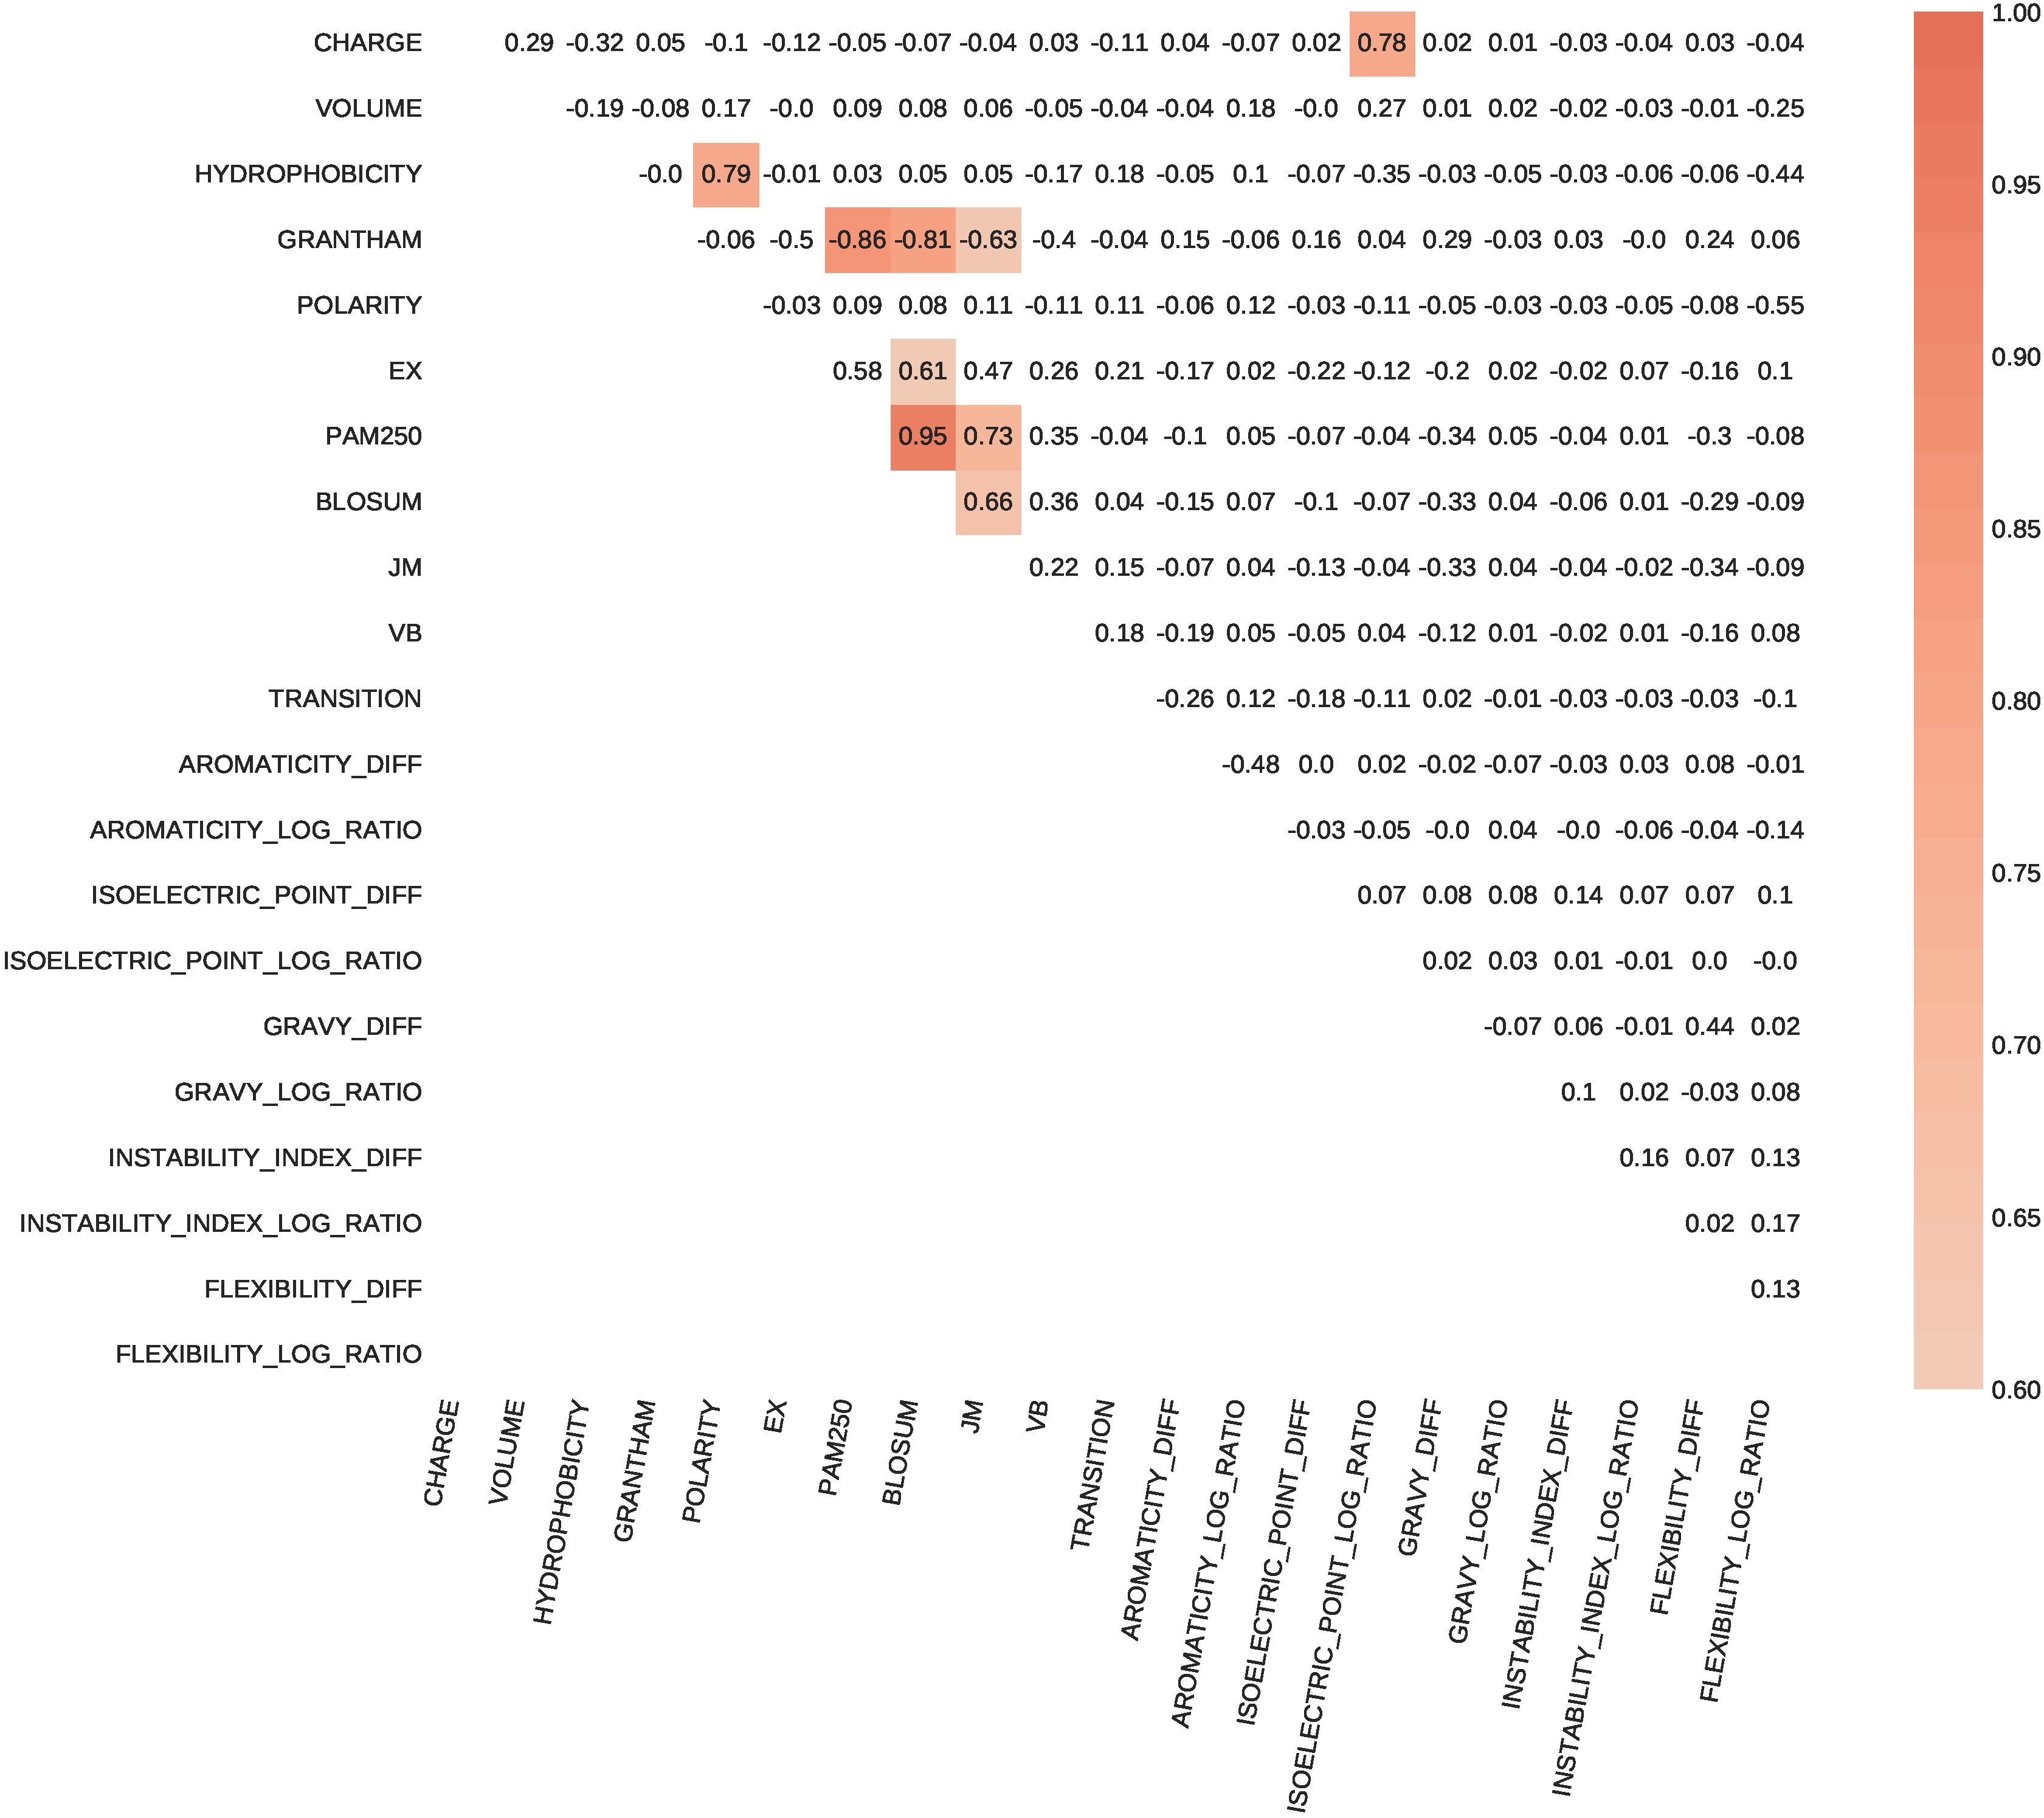
\includegraphics[scale=0.25]{documents/latex/figures/3/structural/structural_corr.pdf}
    \caption{Correlación de Spearman para las variables continuas del dataset Físico-Químico.}
    \label{fig:corrplot_structural}
\end{figure}

Por último, deseamos analizar la correlación entre las variables. Para esto usamos la correlación de Spearman dado que nos permite identificar correlaciones monotónicas. En la figura \ref{fig:corrplot_structural} podemos apreciar un cluster principal de variables altamente correlacionadas: Las matrices de sustitución (GRANTHAM, BLOSUM, JM, y EX). Por otro lado, encontramos a las variables POLARITY e HYDROPHOBICITY correlacionadas entre sí (0.79), como también a las variables CHARGE e ISOELECTRIC\_POINT\_LOG\_RATIO (0.78). Para este análisis decidimos excluir a las variables categóricas por tratarse de variables de tipo binarias con baja cobertura. 


% \subsubsection{Análisis de reducción de dimensionalidad}

% Una de las formas que nos permite ver que tan bien las variables de este dataset están separando nuestros tipos de SNPs, es usar reducción de dimensionalidad. El primer método que probamos fue el análisis de componentes principales (PCA), con el que generamos dos componentes, que son combinaciones lineales de nuestras variables iniciales de forma de maximizar la varianza, es decir el par de componentes que mejor explican la información completa.


% \newpage


\subsection{Generación del modelo}

Con este dataset generamos un modelo basado en un predictor Random Forest. 
Se eligió inicialmente este tipo de predictor por ser el que obtuvo los mejores resultados en el dataset VarQ Curado con respecto a otros predictores (SVMs y Regresión Logística). Otras de las ventajas que aporta este modelo es su facilidad para explicar la importancia de las variables y su relativa baja complejidad computacional, aunque es necesario que tener cuidado a este respecto con las correlaciones presentes entre las variables.

Para generar el modelo volvimos a construir un \textit{pipeline} muy similar al de la sección anterior, que consta de las siguientes etapas:

\begin{itemize}
 
\item \textbf{Imputación}: Las variables, cuyos valores eran nulos, se imputaron usando la mediana en el caso de las variables continuas, y con el valor más frecuente para las variables categóricas. 
\item \textbf{Escalado}: Las variables no fueron escaladas al no ser necesario en algoritmos de clasificacion basados en árboles de decisión, dado que se evalúan las variables de forma independiente. 
\item \textbf{Búsqueda de Hiperparámetros}: Para la búsqueda de hiperparámetros usamos \textit{Grid-Search} (búsqueda ``en cuadrícula'').
\end{itemize}


\subsection{Resultados del modelo Físico-Químico}

Como puede observarse en la figura \ref{fig:auc_structural}, a partir de este modelo se obtuvo un AUC de 0.72, que no supera lo obtenido por el modelo usando el dataset VarQ Curado. Las métricas observadas en la tabla \ref{structural_table} permiten dar cuenta de una precisión del 68\% con respecto a las observaciones patogénicas, es decir, el modelo está reportando un 32\% de variantes como patogénicas que no lo son (también conocido como error de tipo I), y un recall de 47\%, lo que indica que existe un 53\% de variantes patogénicas en nuestro dataset que no están siendo detectadas por nuestro modelo (error de tipo II). 

\begin{table}[H]
\centering
\begin{tabular}{|l|l|l|l|}
\hline
              & Precisión & Recall & F1-score \\ \hline
Benignas      & 0.68      & 0.81   & 0.74     \\ \hline
Patogénicas   & 0.65      & 0.47   & 0.54     \\ \hline
Promedio      & 0.66      & 0.67   & 0.66     \\ \hline
\end{tabular}
\caption{Métricas del modelo Random Forest aplicado al dataset Físico-Químico.}
\label{structural_table}
\end{table}


\subsection{Importancia de los atributos}

El algoritmo Random Forest nos permite identificar los mejores atributos en cada uno de los árboles del clasificador. En este caso, los primeros cuatro atributos refieren a matrices de sustitución (figura \ref{fig:importances_structural}). La quinta variable en importancia pertenece a ProtParam (AROMATICITY\_DIFF). 

También en la figura \ref{fig:importances_structural}, se observan variables con un nivel de importancia muy similar, como es el caso de PAM250, EX, BLOSUM y GRANTHAM. Todas estas variables corresponden a matrices de sustitutción, por lo que no es de extrañar que también exista un alto nivel de correlación entre ellas (ver figura \ref{fig:corrplot_structural}). 

Para analizar el impacto de clusters de variables altamente correlacionadas, usamos la herramienta \texttt{rfpimp} desarrollada por Terrence Parr y otros. Esta herramienta permite agrupar variables y analizar su importancia realizando permutaciones sobre las variables escogidas y reportando la perdida de precisión en el modelo. En la figura \ref{fig:importances_structural_cluster} vemos como las variables de hidrofobicidad y polaridad se ubican a la par de la matriz GRANTHAM. También aparecen nuevas variables en nivel de importancia, como DNA\_BIND y TRANSMEM (Sitio de unión de la proteína y region transmembrana respectivamente).


\pagebreak

\begin{figure}[H]
\centering
\begin{subfigure}[b]{0.7\textwidth}
    \centering
    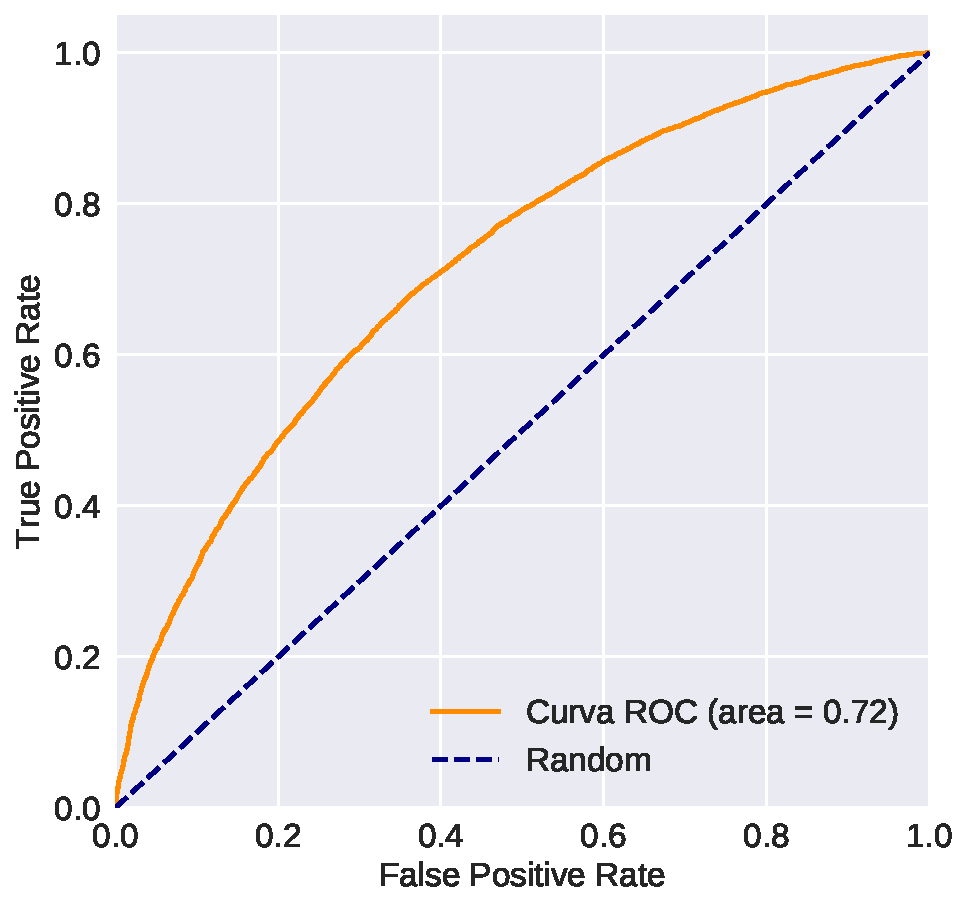
\includegraphics[width=\textwidth]{documents/latex/figures/3/structural/auc_structural.pdf}
    \caption{Curva AUC del algoritmo Random Forest aplicado al dataset Físico-Químico. La línea punteada corresponde a un predictor Random.}
    \label{fig:auc_structural}
\end{subfigure}

\hfill
\hfill

\begin{subfigure}[b]{0.7\textwidth}
    \centering
    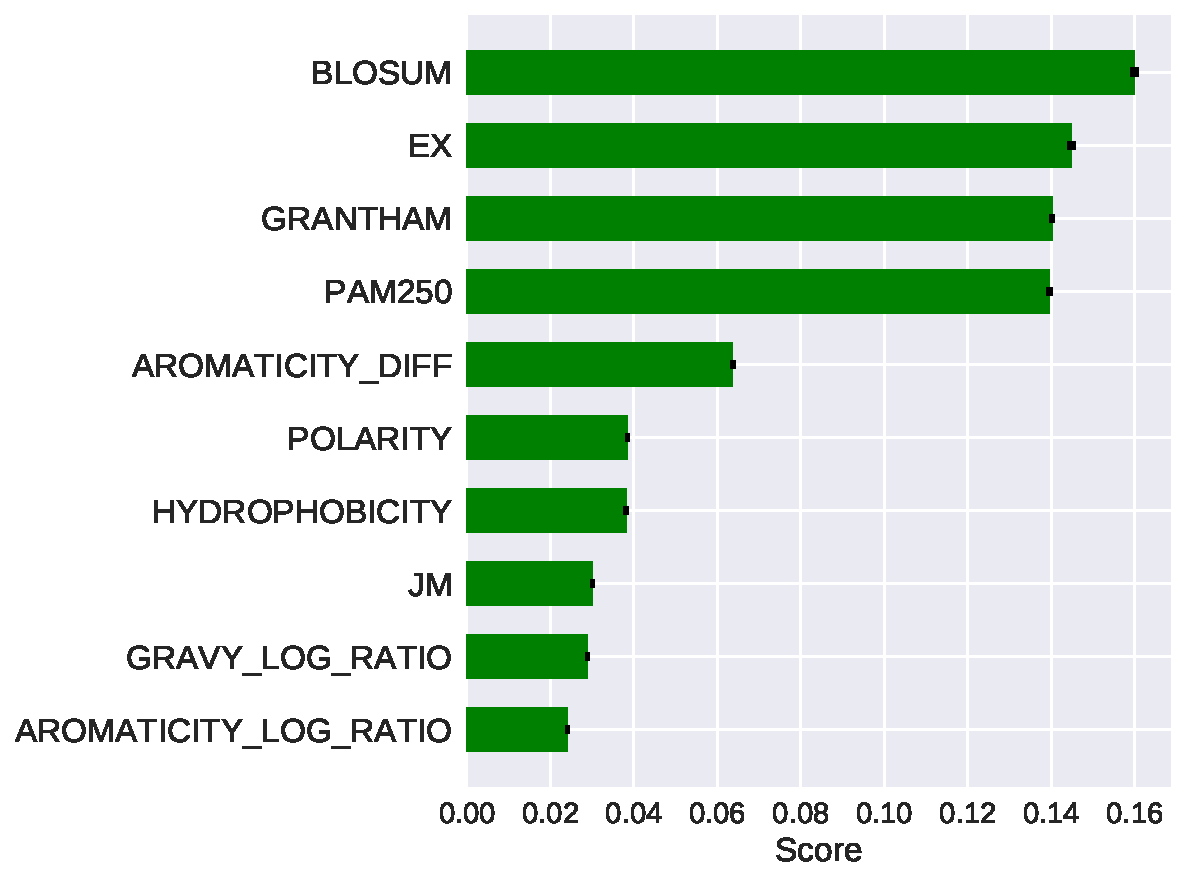
\includegraphics[width=\textwidth]{documents/latex/figures/3/structural/importances_structural.pdf}
    \caption{Los 10 atributos más importantes del modelo Random Forest usando el dataset Físico-Químico.}
    \label{fig:importances_structural}
\end{subfigure}

\caption{Curva AUC y atributos más importantes del modelo Físico-Químico}
\end{figure}

\newpage

\begin{figure}[H]
    \centering
    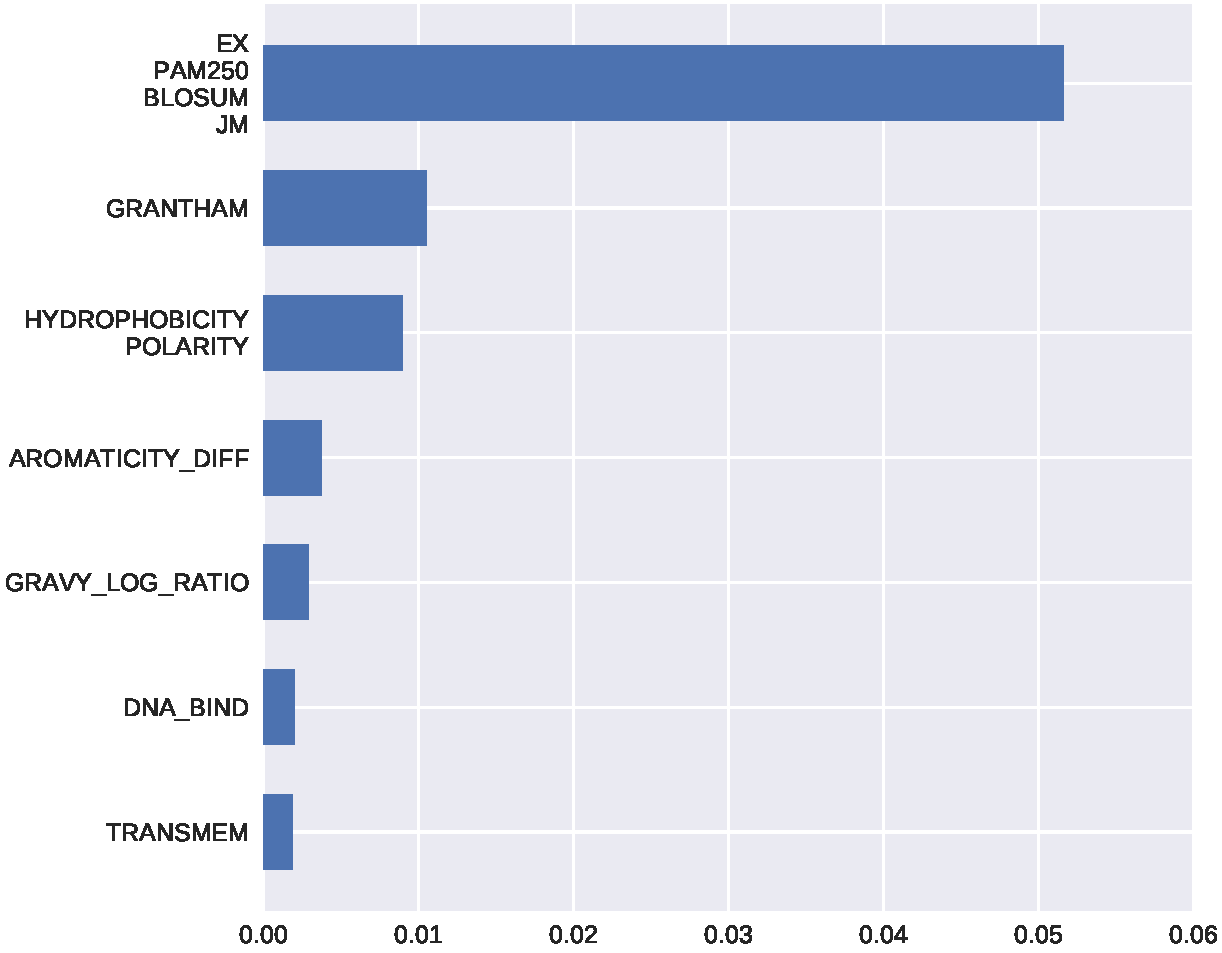
\includegraphics[scale=0.6]{documents/latex/figures/3/structural/structural_importance_cluster.pdf}
    \caption{Variación en la precisión al permutar clusters de variables correlacionadas ($>$ 0.90) del dataset Físico-Químico.}
    \label{fig:importances_structural_cluster}
\end{figure}


\section{Modelo usando variables genómicas}

Otra de las preguntas que nos hicimos fue si las variables genómicas podían hacer un aporte al modelo, siendo que es en los genes donde se produce la mutación que finalmente da origen a la variante en la proteína. En la base de datos Humsavar existe, para la mayoría de las mutaciones, el identificador rsID o Reference SNP ID. Un identificador rsID agrupa los distintos reportes que hacen referencia a la misma posición dentro del mismo genoma de referencia (hg19/GRCh37, en nuestro caso). A partir de este identificador fue posible obtener de la base de datos dbSNP (Versión snp150) \cite{dbSNP}, datos como el cromosoma, la posición, el cambio de nucleótido de la variante y su clasificacion funcional.

\subsection{Variables de conservación}

En la literatura encontramos que dos de las variables genómicas asociadas a la conservación eran las que daban mejores resultados (modelos FATHMM-MKL \cite{Shihab2015} o VEST \cite{Carter2013}). La \textit{conservación} es un concepto biológico que refiere a las secuencias conservadas, es decir, secuencias tanto genéticas como proteicas que se mantienen de forma similar o idéntica en muchas especies que poseen un ancestro evolutivo en común. La conservación puede ser cuantificada con distintos tipos de enfoques, pero en lo que nos concierne, dos de los más utilizados son 1) a través de alineamientos múltiples de secuencias y 2), mediante el uso de árboles filogenéticos.

En particular, la composición de estas variables consiste en alineamientos múltiples de secuencias genéticas (MSA) de 46 especies de vertebrados, incluyendo Homo Sapiens y otras como Felis catus (gato doméstico), Danio renus (pez cebra) y Equus Caballus (caballo). En base a este alineamiento se usan dos medidas distintas que buscan detectar aquellas regiones en el genoma (ADN) con mayor nivel de conservación entre las distintas especies. Las medidas son las siguientes:
\begin{itemize}
    \item \textbf{PhastCons-46-Way} \cite{siepel2005evolutionarily}: Medida de conservación basado en un modelo oculto de Markov (\textit{phylo-HMM}). Calcula la probabilidad de que un nucleótido pertenezca a un sitio conservado (considerando el entorno).
    \item \textbf{PhyloP-46-Way} \cite{Pollard2010}: mide la conservación en una columna individual, sin considerar las columnas vecinas.
\end{itemize}

Decidimos incluir en nuestro dataset ambas medidas de conservación, usando el Table Browser de la Universidad de California en Santa Cruz (UCSC) \cite{Karolchik2004}.

\subsection{Variables relativas a la clase funcional}

También tomamos en consideración la función de la posición dentro del gen. La base de datos dbSNP define cada SNP de acuerdo a su clase funcional. Si la variación se encuentra cerca del intervalo de un transcripto, pero no en la región codificante, la clase funcional va a depender de la posición de la variación relativa a la estructura del transcripto \cite{Ostell2007}.  Por otro lado, si la variación se encuentra en una zona codificante, la clase funcional se va a definir en base a si el alelo de la variación va a resultar en una sustitución sinónima (es decir, el nuevo codón va a formar el mismo aminoácido), una sustitución no sinónima (es decir, el nuevo codón va a formar un aminoácido distinto) o una sustitución sin sentido (en donde la mutación genera un codón de terminación prematuro). En base a esta información generamos variables binarias, que indican con 1 ó 0 la existencia de un lugar con una determinada clase funcional.


% , que puede ser:
 
% \begin{itemize}
%     \setlength\itemsep{0em}
%     \item INTRON
%     \item MISSENSE
%     \item NEAR-GENE
%     \item NCRNA
%     \item CODING-SYNON
%     \item UNTRANSLATED
%     \item NONSENSE
%     \item SPLICE
%     \item STOP-LOSS
% \end{itemize}

\subsection{Extracción de variables usando SNVBox}

Por último, usamos variables genómicas del dataset SNVBox, específicamente de la tabla \\ EXON\_FEATURES. Las variables usadas son:
\begin{itemize}
    \item ExonConservation (CONS): Score de Conservación para el exón completo calculado a partir de una alineación filogenética a 46 vías, usando el \textit{Genome Browser}. Si bien existe una gran similitud con las variables de conservación que ya incluimos en el dataset decidimos incluir esta variable debido a su baja correlación con las mencionadas anteriormente (ver descripción estadística del dataset).
    \item ExonHapMapSnpDensity (HAPMAP\_SNP\_DEN): Número de SNPs (verificados en HapMap) en el exón donde ocurre la mutación dividido por la longitud del exón. Estos SNPs (también llamados tag SNPs) son los que identifican haplotipos. Los haplotipos son bloques de SNPs heredados por un único individuo.
    \item ExonSnpDensity (SNP\_DEN): Número de SNPs en el exón donde ocurre la mutación dividido por la longitud del exón.
\end{itemize}

Estas variables se definen a nivel de exón, por lo que cada una de ellas posee dos identificadores: UID (identificador de la secuencia proteica a la que pertenece) y EXON (identificador del exón dentro de cada transcripto mRNA). Estos identicadores permiten el cruce con la tabla \texttt{Transcript\_Exon} dentro de la base SNVBox. Con esta tabla podemos obtener el número del cromosoma del exón, y la posición de inicio y fin del exón dentro del cromosoma. Una vez obtenidos estos datos, pudimos extraer todos los rsID dentro de esa subsecuencia. Finalmente, le asignamos el valor de la variable a todos los rsIDs en nuestra tabla Humsavar. Para algunos casos obtuvimos más de un valor para un mismo rsID, por lo que tomamos la decisión de promediarlos.

\todo{Esquema de acceso a la variable}

\subsection{Construcción del dataset Genómico}

Con los atributos mencionados anteriormente, pudimos cruzar la información usando la columna rsID (Reference SNP cluster ID). Esta columna identifica a un cluster de variaciones de un sólo nucleótido que pertenece a la misma posición en el genoma (o conjunto de posiciones) \cite{Ostell2007}. Filtramos las variantes de Humsavar que no poseían este identificador. Finalmente el dataset Genómico se compone de 55,382 variantes de las cuales 37,572 (68\%) son benignas y 17,807 (32\%) son patogénicas. 

\subsection{Descripción estadística del dataset Genómico}

A continuación presentamos, como en las secciones anteriores, una descripción de las variables usadas (tablas \ref{conservacion_vars} y \ref{snvbox_vars}). Para cada uno de los grupos analizamos la media (mean), el desvío estándar (std), los cuartiles (25\%, 50\%, 75\%) y los valores máximos (max) y mínimos (min). También incluimos el AUC univariado y el \textit{Balanced Accuracy} para las variables categóricas, en este caso las relativas a la clase funcional (tablas \ref{conservacion_vars} y \ref{snvbox_vars}). El AUC univariado de las variables de conservación (PHYLOP46WAY, PHASTCONS46WAY y CONS) es alto, lo que significa que variantes en zonas de alta conservación son buenos indicadores de patogenicidad.

% \subsubsection{Variables de Conservación}
\begin{table}[H]
\centering
\begin{tabular}{|l|l|l|l|l|l|l|l|l|}
\hline
Variable & mean & std & min & 25\%  & 50\% & 75\%  & max & AUC \\ \hline
PHYLOP46WAY & 2.16 &  2.29 & -8.22 &  0.29 &  1.81 &  4.23 &  6.42 & 0.83 \\ \hline
PHASTCONS46WAY & 0.67 & 0.44 &  0.00 &  0.06 &  0.99 &  1.00 &  1.00 & 0.78 \\ \hline
\end{tabular}
\caption{Variables de Conservación del dataset Genómico.}
\label{conservacion_vars}
\end{table}

% \subsubsection{}
\begin{table}[H]
\centering
\begin{tabular}{|l|l|l|l|l|l|l|l|l|}
\hline
Variable         & mean & std  & min  & 25\% & 50\% & 75\% & max & AUC  \\ \hline
CONS             & 0.65 & 0.09 & 0.14 & 0.59 & 0.66 & 0.72 & 0.90 & 0.65 \\ \hline
SNP\_DEN         & 0.06 & 0.10 & 0.00 & 0.03 & 0.04 & 0.06 & 1.04 & 0.56 \\ \hline
HAPMAP\_SNP\_DEN & 0.00 & 0.00 & 0.00 & 0.00 & 0.00 & 0.00 & 0.04 & 0.48 \\ \hline
\end{tabular}
\caption{Variables extraídas de SNVBox a nivel de Exón}
\label{snvbox_vars}
\end{table}

% \subsubsection{Variables relativas a la Clase Funcional}
% \begin{table}[H]
% \begin{tabular}{|l|l|l|l|l|l|l|l|l|}
% \hline
% Variable     & count    & mean & std  & min  & 25\% & 50\% & 75\% & max  \\ \hline
% INTRON       & 54849.00 & 0.14 & 0.34 & 0.00 & 0.00 & 0.00 & 0.00 & 1.00 \\ \hline
% MISSENSE     & 54849.00 & 0.99 & 0.10 & 0.00 & 1.00 & 1.00 & 1.00 & 1.00 \\ \hline
% NEAR-GENE    & 54849.00 & 0.06 & 0.24 & 0.00 & 0.00 & 0.00 & 0.00 & 1.00 \\ \hline
% NCRNA        & 54849.00 & 0.17 & 0.38 & 0.00 & 0.00 & 0.00 & 0.00 & 1.00 \\ \hline
% CODING-SYNON & 54849.00 & 0.02 & 0.14 & 0.00 & 0.00 & 0.00 & 0.00 & 1.00 \\ \hline
% UNTRANSLATED & 54849.00 & 0.05 & 0.23 & 0.00 & 0.00 & 0.00 & 0.00 & 1.00 \\ \hline
% NONSENSE     & 54849.00 & 0.01 & 0.07 & 0.00 & 0.00 & 0.00 & 0.00 & 1.00 \\ \hline
% SPLICE       & 54849.00 & 0.00 & 0.02 & 0.00 & 0.00 & 0.00 & 0.00 & 1.00 \\ \hline
% STOP-LOSS    & 54849.00 & 0.00 & 0.01 & 0.00 & 0.00 & 0.00 & 0.00 & 1.00 \\ \hline
% \end{tabular}
% \end{table}


% \subsubsection{Correlación entre las variables}

Como era de esperarse, la figura \ref{fig:corrplot_genomic} muestra una alta correlación entre las variables de conservación phyloP y phastCons (0.82). Por otro lado, la correlación entre HAPMAP\_SNP\_DEN y SNP\_DEN es muy baja (0.06), pese a que su construcción es muy similar. Esto se debe a la diferencia entre la cantidad total de SNPs en un humano (alrededor de 10 millones) comparados con los que se encuentran en HapMap (~500,000 en total).

\begin{figure}[H]
    \centering
    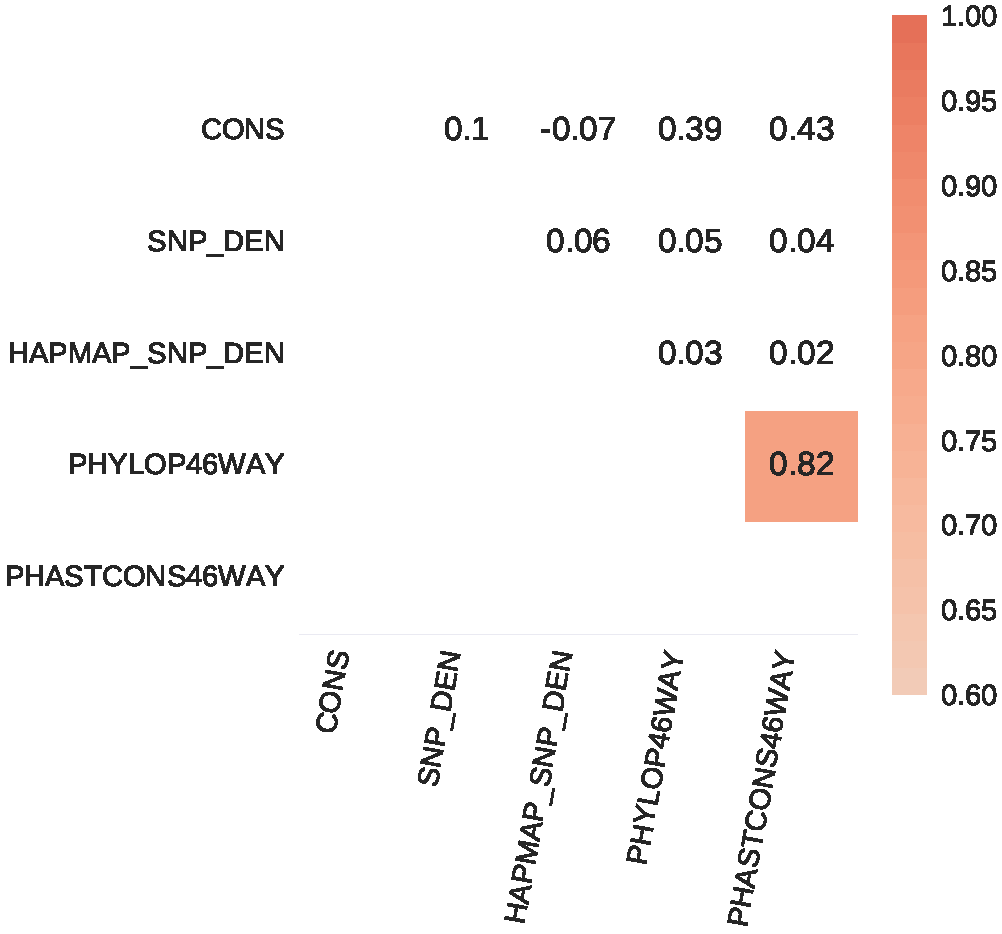
\includegraphics[scale=0.5]{documents/latex/figures/3/genomic/genomic_corr.pdf}
    \caption{Correlación de Spearman para las variables continuas del dataset Genómico.}
    \label{fig:corrplot_genomic}
\end{figure}

% \newpage

\subsection{Generación del Modelo}

Luego de realizada la exploración del dataset Genómico generamos un modelo basado en Random Forest. Volvimos a utilizar este algoritmo debido a los resultados obtenidos en el dataset VarQ Curado y para facilitar la comparación entre los datasets estudiados. Este modelo se compone de un \textit{pipeline} de dos fases principales: Imputación y Entrenamiento. En la fase de imputación se reemplazaron los valores nulos por el valor más frecuente, en el caso de las variables categóricas (por ejemplo las referentes a las clases funcionales) y con la mediana para las variables continuas. Las variables no fueron escaladas dado que en los algoritmos que involucran árboles de decisión, como Random Forest, las variables son evaluadas una a una y por lo tanto la escala de cada una de ellas no afecta la evaluación de las demás.

\subsection{Resultados del modelo genómico}

Como se puede observar en la figura \ref{fig:auc_genomic} obtuvimos un AUC de 0.85. Este resultado es muy superior a los obtenidos en los modelos anteriores, tanto en VarQ Curado como el dataset Físico-Químico. En la tabla \ref{tab:metrics_genomic} vemos los valores de \textit{precision}, \textit{recall} y \textit{f1-score} para las dos clases. En este caso podemos advertir una mejora total en cada una de las métricas comparándolas con las obtenidas en base al modelo Físico-Químico. En particular destacamos la mejora en precisión de la detección de variables benignas, que pasó de un 0.68 en el modelo Físico-Químico a un 0.83 en el modelo Genómico, es decir un 15\% de mejora; como así también el crecimiento en el \textit{recall} de variantes patogénicas, que saltó de un 0.47 en el modelo Físico-Químico a un 0.64, lo que representa un 17\% de mejora.

\begin{table}[H]
\centering
\begin{tabular}{|l|l|l|l|}
\hline
             & precision & recall & f1-score \\ \hline
Benignas     & 0.83      & 0.87   & 0.85     \\ \hline
Patogénicas  & 0.69      & 0.64   & 0.67     \\ \hline
Promedio     & 0.79      & 0.79   & 0.79     \\ \hline
\end{tabular}
\caption{Reporte de métricas del modelo Random Forest usando el dataset Genómico.}
\label{tab:metrics_genomic}
\end{table}

% Otra de las razones que explican esta diferencia es la forma en que son calculadas. El dataset VarQ usa una variable basada a nivel de proteínas 


\subsection{Importancia de los atributos}
Analizando la importancia de las variables en el modelo, en la figura \ref{fig:importances_genomic} podemos observar que las variables de conservación (phastCons y phyloP) están en los primeros dos puestos, confirmando lo obtenido por los trabajos de investigación antes mencionados. 

El poder informativo sumado de estas variables equivale a un porcentaje superior al 80\% de la importancia total. La pregunta que nos hacemos en este caso es: ¿Las dos primeras variables de conservación están en los primeros dos lugares porque están altamente correlacionadas o aportan diferente información sobre las variables? En la figura \ref{fig:corrplot_genomic} podemos observar que estas variables se encuentran muy correlacionadas (0.82), lo que sugiere un alto grado de redundancia. En la figura \ref{fig:importance_genomic_cluster}, observamos que esta proporción se mantiene al agrupar en clusters a las variables correlacionadas.

Por otro lado, esto genera un interrogante adicional: ¿Cuál es la razón por la que la variable \textit{Conservación} del dataset VarQ Curado no genera un rendimiento similar? Una de las principales razones que encontramos es en el nivel de cobertura de la variable. En el caso de las variables de conservación genómica, la cobertura de las mismas llega a un nivel superior al 95\%, mientras que en el caso de la conservación en el dataset VarQ Curado este número no llega al 40\%.  Otra razón posible a considerar tiene que ver con la naturaleza del cálculo de conservación de VarQ via PFAM, que contiene una heterogeneidad muy grande de especies (alrededor de 16,000 familias), y se basa en secuencias de proteínas.

\begin{figure}[H]
    \centering
    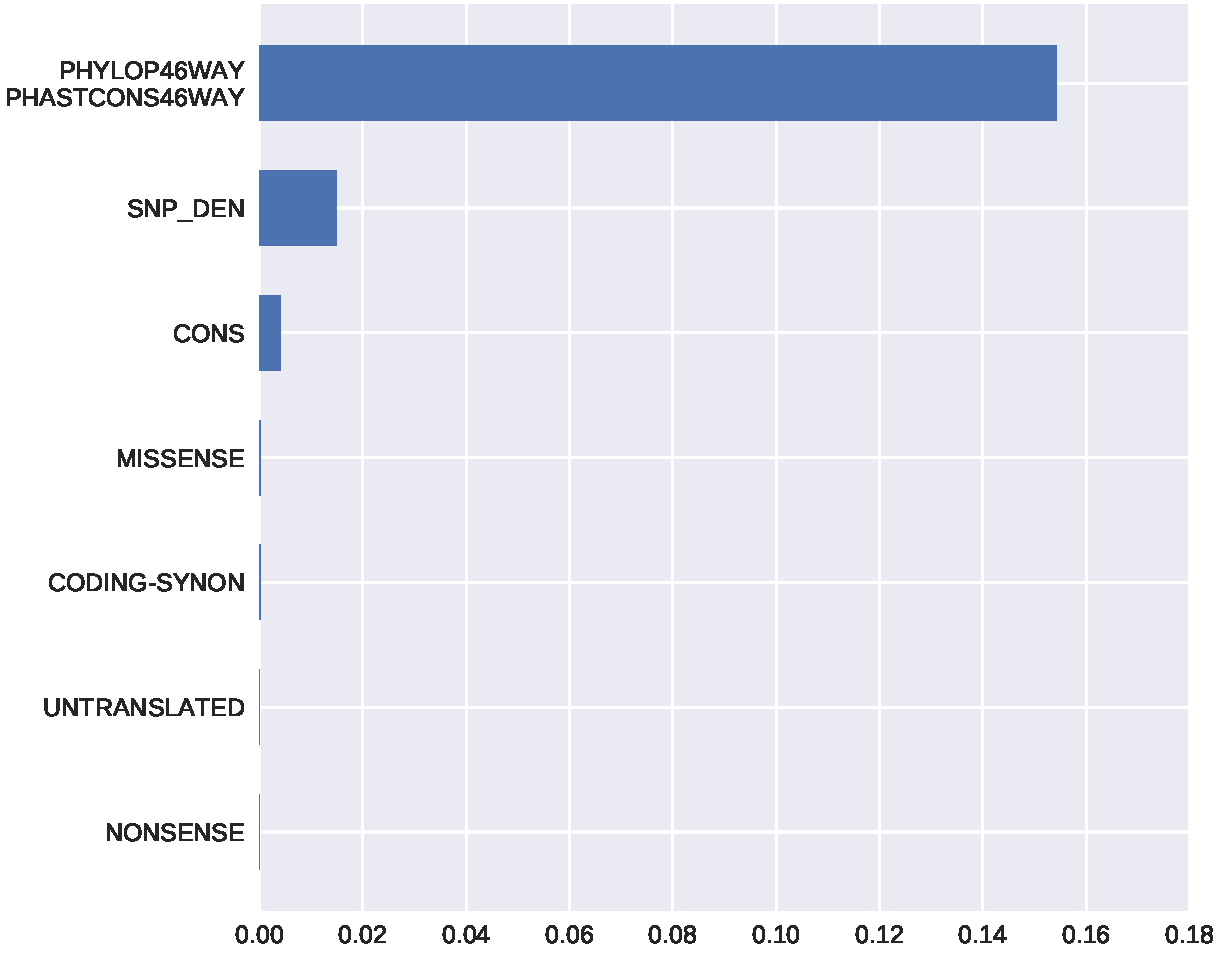
\includegraphics[scale=0.5]{documents/latex/figures/3/genomic/genomic_importance_cluster.pdf}
    \caption{Variación en la precisión al permutar clusters de variables correlacionadas ($>$ 0.90) del dataset Genómico.}
    \label{fig:importance_genomic_cluster}
\end{figure}


\newpage

\begin{figure}[H]
\centering
\begin{subfigure}[b]{0.7\textwidth}
    \centering
    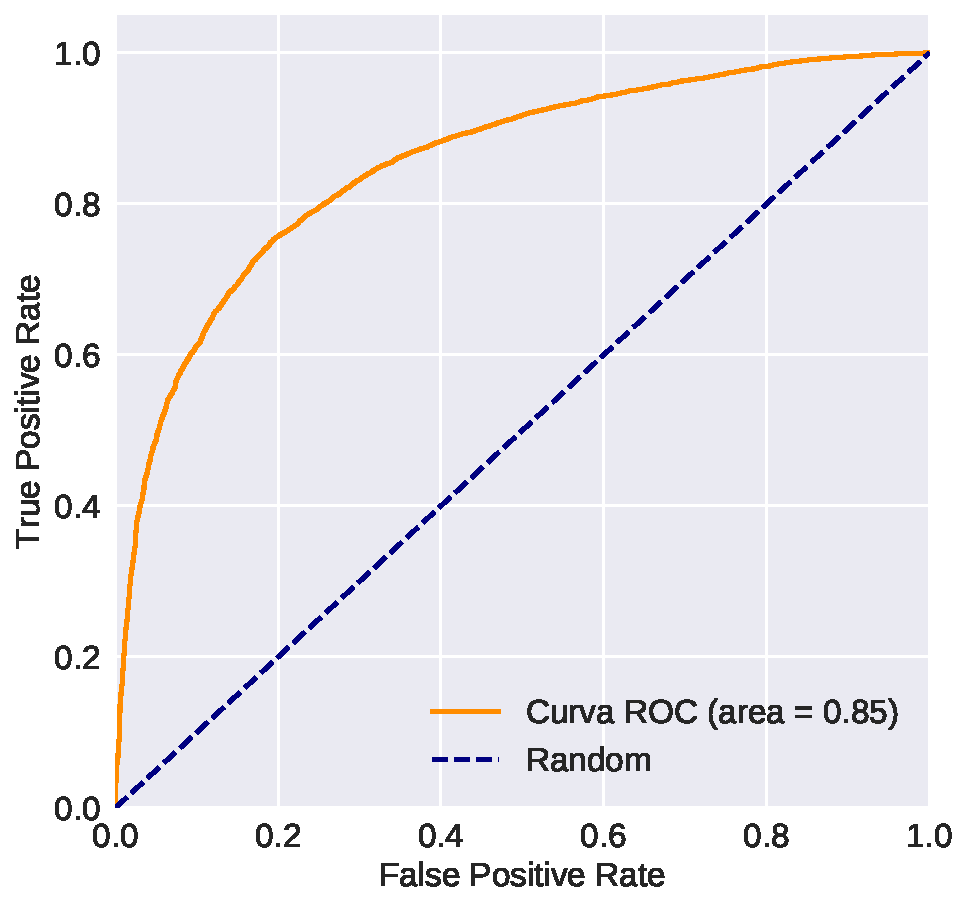
\includegraphics[width=\textwidth]{documents/latex/figures/3/genomic/auc_genomic.pdf}
    \caption{Curva AUC del algoritmo Random Forest aplicado al dataset Genómico. La línea punteada corresponde a un predictor Random.}
    \label{fig:auc_genomic}
\end{subfigure}

\hfill
\hfill

\begin{subfigure}[b]{0.7\textwidth}
    \centering
    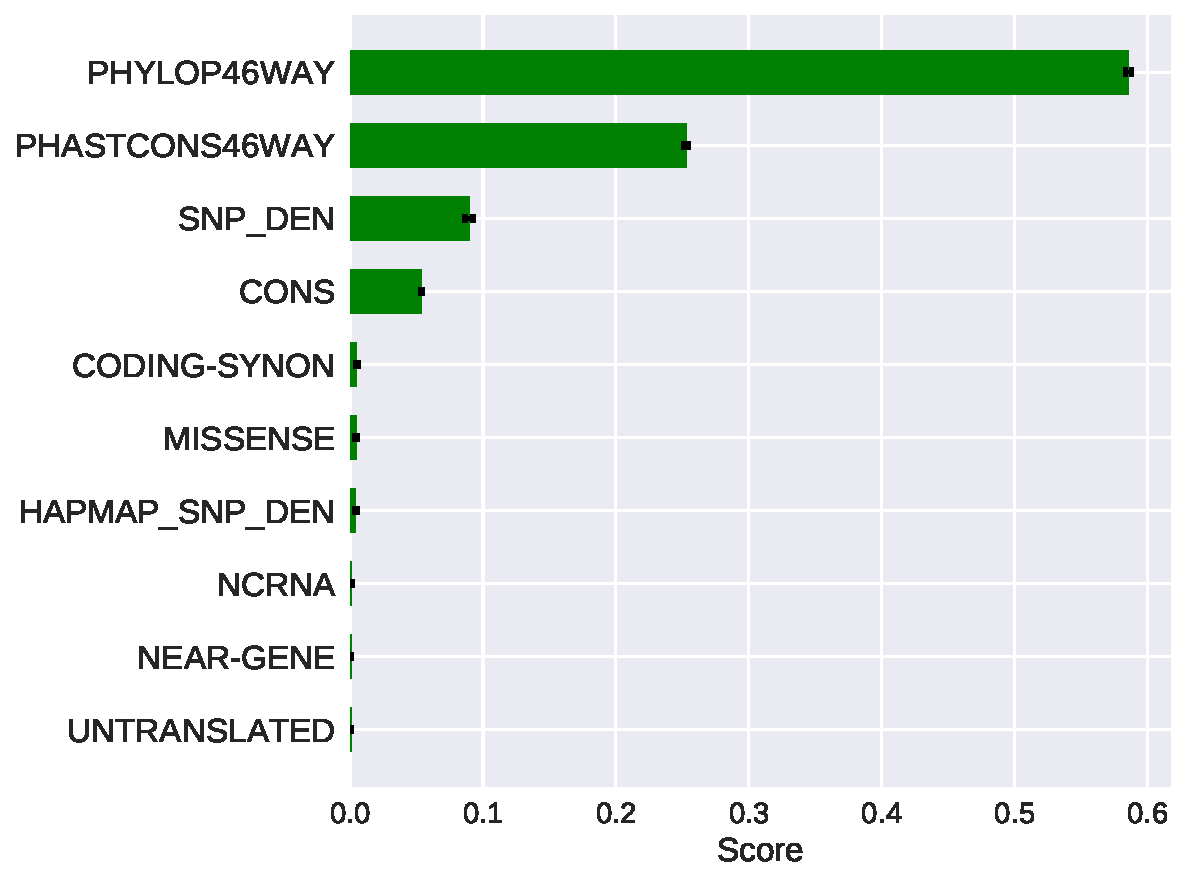
\includegraphics[width=\textwidth]{documents/latex/figures/3/genomic/importances_genomic.pdf}
    \caption{Los 10 atributos más importantes del modelo Genómico.}
    \label{fig:importances_genomic}
\end{subfigure}

\caption{Curva AUC y atributos más importantes del modelo Genómico.}

\end{figure}

\newpage

% \subsection{Descripción}
% \subsection{Correlación}
% \subsection{Resultados}

\section{Integrando el dataset Físico-Químico y el Genómico}

Finalmente, unimos los dos conjuntos de variables para evaluar si la integración de ambos datasets representan una mejora frente a los resultados del modelo Genómico y Físico-Químico por separado. A este nuevo dataset lo denominamos dataset Integral. Las variantes usadas fueron nuevamente las encontradas en la tabla Humsavar. 

\subsection{Creación del dataset Integral}

El dataset Integral posee 68,508 variantes (la misma cantidad de variantes del dataset Físico-Químico), con 64 variables, que son las variables sumadas de los datasets Genómico (14), Físico-Químico (49) y la variable de respuesta. Del total de las variantes, 39,653 (58\%) son benignas y 28,855 (42\%) son patogénicas. 

\subsection{Generación del modelo}

Para este modelo preliminar utilizamos nuevamente el algoritmo Random Forest, repitiendo las mismas fases de imputación y entrenamiento usadas previamente en los modelos Genómico y Físico-Químico. Es decir, que en la fase de imputación usamos la mediana para los valores nulos de las variables continuas y el valor más frecuente en las variables categóricas. El entrenamiento consistió en una búsqueda de hiperparámetros óptimos usando \textit{GridSearch} en un diccionario de posibles parámetros, evaluados en una triple validación cruzada basándonos en el AUC como métrica a optimizar. El dataset de entrenamiento posee 45,900 variantes, aproximadamente dos tercios del dataset completo. Una vez entrenado el modelo usando este \textit{pipeline}, se evaluaron las variantes del dataset de testeo, es decir, el tercio restante del dataset completo. Posteriormente utilizamos un método de boosting, Extreme Gradient Boosting (xgboost). Los hiperparámetros de este método fueron elegidos usando una búsqueda randomizada (Randomized Grid Search). Este método de optimización fue elegido dado que las combinaciones que se evalúan en el método Grid Search son demasiadas. La búsqueda randomizada evalúa las mismas alternativas pero eligiendo combinaciones de forma aleatoria, sin probar todas las combinaciones. También es posible evaluar valores tomados de acuerdo a una distribución específica.

\subsection{Resultados del modelo Integral [\todo{Faltan resultados de xgboost}]}

El modelo obtuvo un AUC de 0.88. Esto representa una mejora con respecto al modelo Genómico (0.85) y al modelo Físico-Químico (0.72). Si comparamos las métricas obtenidas en el modelo Genómico con las de este modelo (figura \ref{tab:metrics_integral}), se puede apreciar un nuevo salto en el \textit{recall} de las variables patogénicas, que pasa de un 0.64 en el modelo Genómico al 0.80, lo que representa un 16\% de mejora. También mejora la precisión con respecto a la detección de esta clase, que pasa de 0.69 a 0.76. La única métrica que decae es el \textit{recall} de la clase Benigna, que pasa de 0.87 a 0.82, lo que representa una leve caída del \textit{f1-score}.

\begin{table}[H]
\centering
\begin{tabular}{|l|l|l|l|}
\hline
Clase        & precision & recall & f1-score \\ \hline
Benignas     & 0.85      & 0.82   & 0.83     \\ \hline
Patogénicas  & 0.76      & 0.80   & 0.78     \\ \hline
Promedio     & 0.81      & 0.81   & 0.81     \\ \hline
\end{tabular}
\caption{Reporte de métricas del modelo Random Forest usando el dataset Integral.}
\label{tab:metrics_integral}
\end{table}


\subsection{Importancia de las variables}

Pasamos a analizar las importancias descriptas en la figura \ref{fig:importances_integral}. Nuevamente encontramos en primer lugar a las variables de conservación genómicas, resultado esperable dado su nivel de importancia en el dataset Genómico y su nivel de AUC conseguido. También encontramos en un segundo escalón a las variables de conservación a nivel de exones, y a una variable que considera el número de SNPs en el exón donde ocurre la mutación. Luego encontramos al grupo de matrices de sustitución de aminoácidos (EX, GRANTHAM, BLOSUM y PAM250), que también aparecieron en los primeros lugares en el modelo Físico-Químico. Por último encontramos una variable relativa a la clase funcional a nivel genómico (MISSENSE) y otra relativa al cambio de polaridad del aminoácido donde ocurre la variante (POLARITY), por lo que encontramos en nuestro ranking una lista de variables transversal a los dos datasets usados. 

En la figura \ref{fig:importance_cluster_integral} unimos las variables de alta correlación en clusters y evaluamos su impacto en la precisión del modelo es la matriz GRANTHAM.



% Dada la alta correlación entre algunas variables que observamos en los modelos anteriores, en esta ocasión 


\begin{figure}[H]
    \centering
    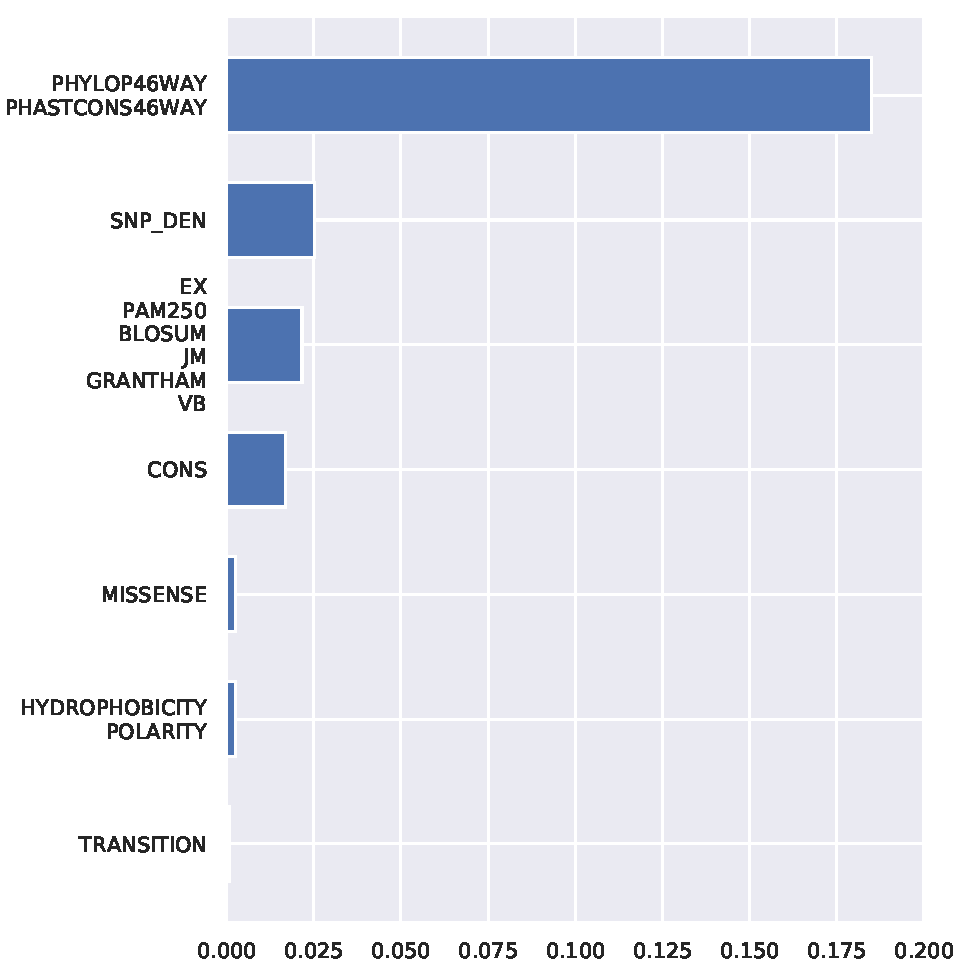
\includegraphics[scale=0.6]{documents/latex/figures/3/integral/integral_importance_cluster.pdf}
    \caption{Importancia de variables clusterizadas (basados en correlación de Spearman) usando permutación.}
    \label{fig:importance_cluster_integral}
\end{figure}

\newpage

\begin{figure}[H]
\centering
\begin{subfigure}[t]{0.7\textwidth}
    \centering
    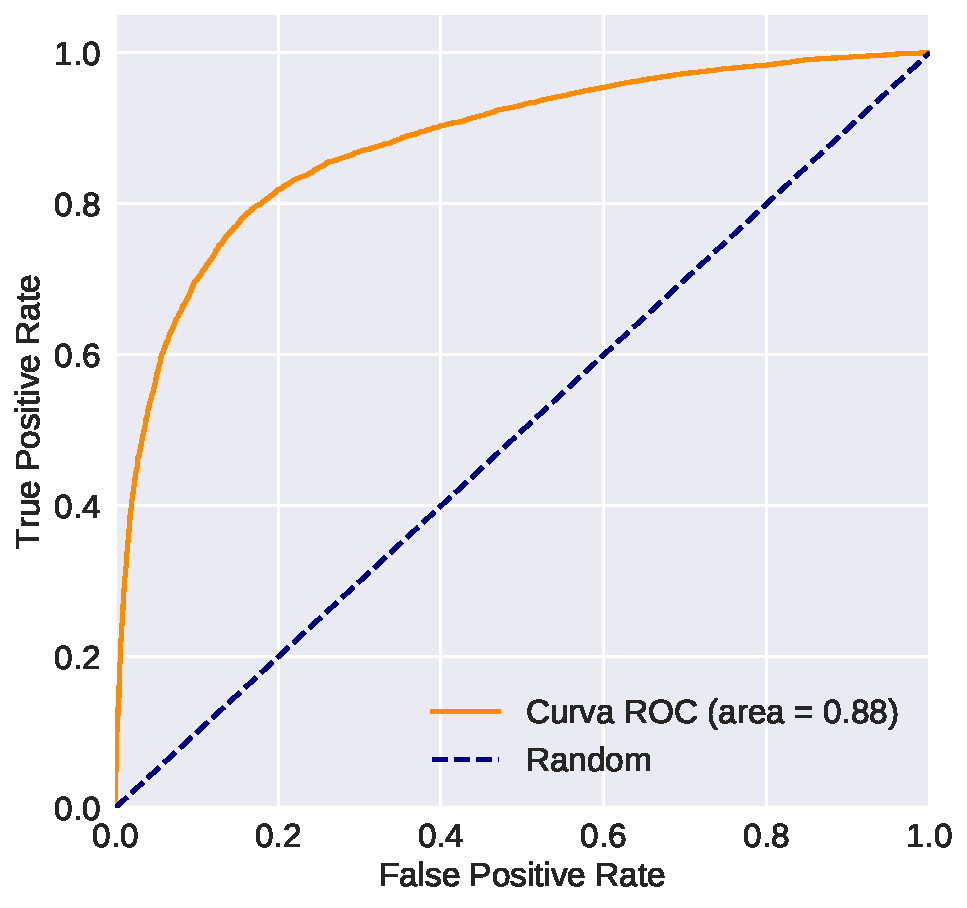
\includegraphics[width=\textwidth]{documents/latex/figures/3/integral/auc_integral.pdf}
    \caption{Curva AUC del algoritmo Random Forest del dataset Integral. La línea punteada corresponde a un predictor Random.}
    \label{fig:auc_integral}
\end{subfigure}
\hfill
\hfill
\begin{subfigure}[b]{0.7\textwidth}
    \centering
    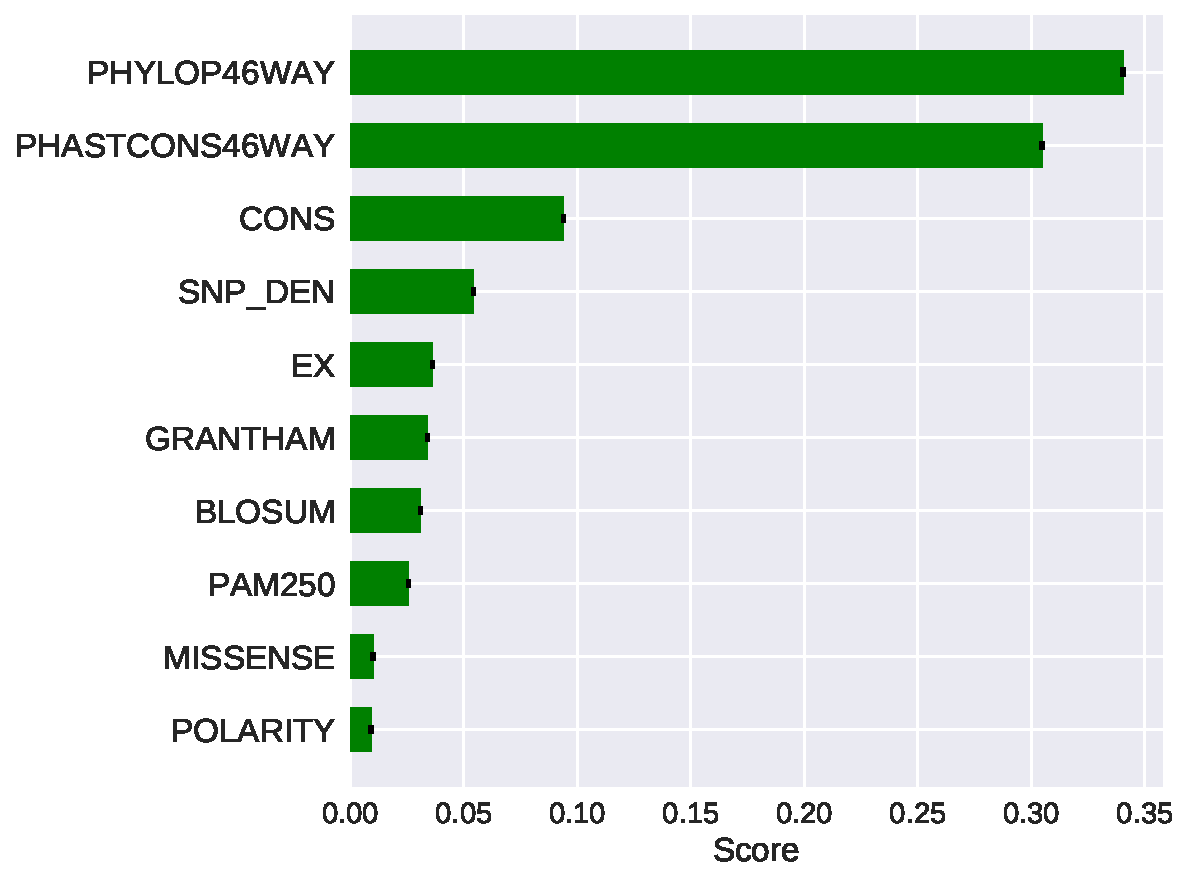
\includegraphics[width=\textwidth]{documents/latex/figures/3/integral/importances_integral.pdf}
    \caption{Los 10 atributos más importantes del dataset Integral.}
    \label{fig:importances_integral}
\end{subfigure}

\end{figure}

\section{Integrando las nuevas variables al dataset VarQ Curado}

En esta sección buscamos cuantificar en qué medida el esfuerzo realizado a lo largo de esta tesis mejora e impacta sobre nuestro set de datos original (VarQ). Para ello, integraremos al set VarQ Curado, que dispone de 9 features estructurales y 7,418 variantes, los features fisico-químicos y genómicos obtenidos a lo largo de esta tesis.

\subsection{Creación del dataset Integral+VarQ Curado}
Para generar este dataset cruzamos las variantes de ambos datasets quedándonos con las variantes de VarQ. El dataset resultante posee 73 variables, que corresponden a las 63 variables del dataset Integral sumado a las 9 variables del dataset VarQ Curado y la variable de respuesta. Este dataset posee 7,418 variantes de las cuales 5,377 (72\%) son patogénicas y 2,041 (28\%) son benignas. 

\subsection{Generación del Modelo}
Como a lo largo de todo este trabajo, volvimos a repetir el pipeline de Random Forest con imputación de variables continuas con la mediana y con el valor más frecuente en el caso de las variables categóricas. También evaluamos el dataset usando xgboost de la misma forma que con el modelo Integral. El dataset de entrenamiento posee 4,970 variantes (66\%), y el tercio restante se destinó al dataset de test. Estas variables fueron elegidas al azar, con una semilla pseudoaleatoria para poder replicar el experimento.  

\subsection{Resultados  [\todo{Faltan resultados de xgboost}]}
El dataset de test arrojó un AUC de 0.87 para RF y 0.88 con xgboost, que representa una mejora sensible con respecto al modelo realizado con el dataset VarQ Curado (0.74), sin superar lo obtenido por el dataset Integral (0.90 con xgboost). Con respecto a las métricas de análisis, en la tabla \ref{tab:metrics_integral_varq} observamos una mejora generalizada, especialmente en la precisión en la detección de variantes benignas, que pasa de 0.57 a 0.81 en el nuevo modelo, y también en el \textit{recall}, que pasa de 0.26 a 0.53. Si bien sigue siendo un número bajo, es posible modificar el \textit{threshold} en la función de decisión para obtener un \textit{recall} más alto sacrificando precisión. 

\begin{table}[H]
\centering
\begin{tabular}{|l|l|l|l|}
\hline
             & precision & recall & f1-score \\ \hline
Benignas     & 0.81      & 0.53   & 0.64     \\ \hline
Patogénicas  & 0.84      & 0.95   & 0.89     \\ \hline
Promedio     & 0.83      & 0.83   & 0.82     \\ \hline
\end{tabular}
\caption{Reporte de métricas del modelo Random Forest usando el dataset Integral+VarQ Curado.}
\label{tab:metrics_integral_varq}
\end{table}

\subsection{Importancia de las variables}
La información proporcionada por la librería acerca de la importancia de las variables en el modelo \textit{scikit-learn} están presentadas en la figura \ref{fig:importances_integral_varq}. En este ranking de las 10 variables más relevantes encontramos otra vez en primer lugar con amplia ventaja a las variables de conservación genómica, aunque también se mantiene la variación de energía y al porcentaje de SASA, que son variables pertenecientes al dataset VarQ Curado y que habían aparecido en el ranking de dicho modelo. 

\begin{figure}[H]
    \centering
    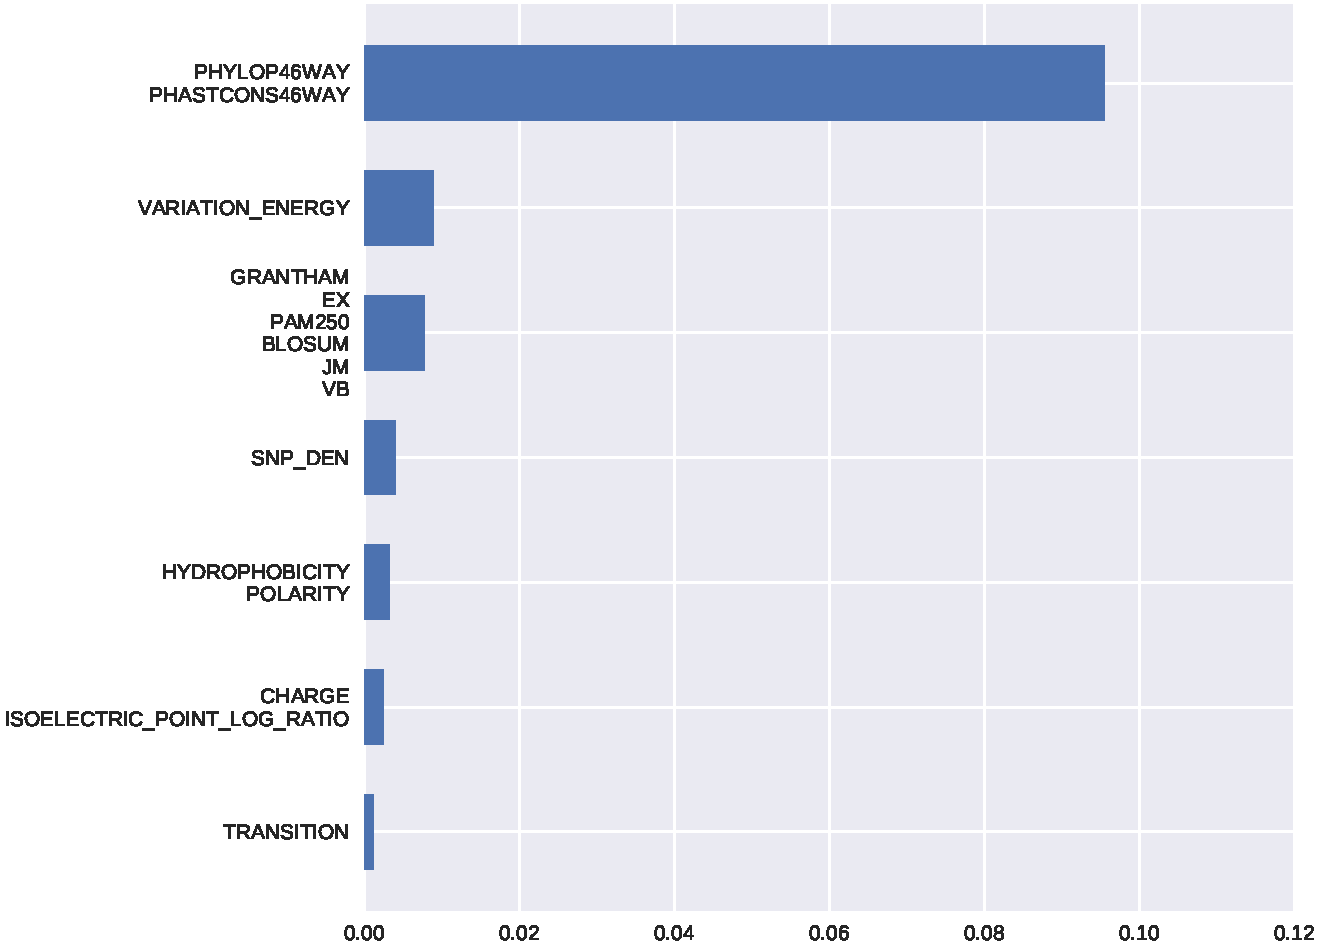
\includegraphics[scale=0.6]{documents/latex/figures/3/integral_varq/integral_varq_importance_cluster.pdf}
    \caption{Variación en la precisión al permutar clusters de variables correlacionadas ($>$ 0.90) del dataset Integral+VarQ Curado.}
    \label{fig:importance_cluster_integral_varq}
\end{figure}


\newpage
\begin{figure}[H]
\centering
\begin{subfigure}[b]{0.7\textwidth}
    \centering
    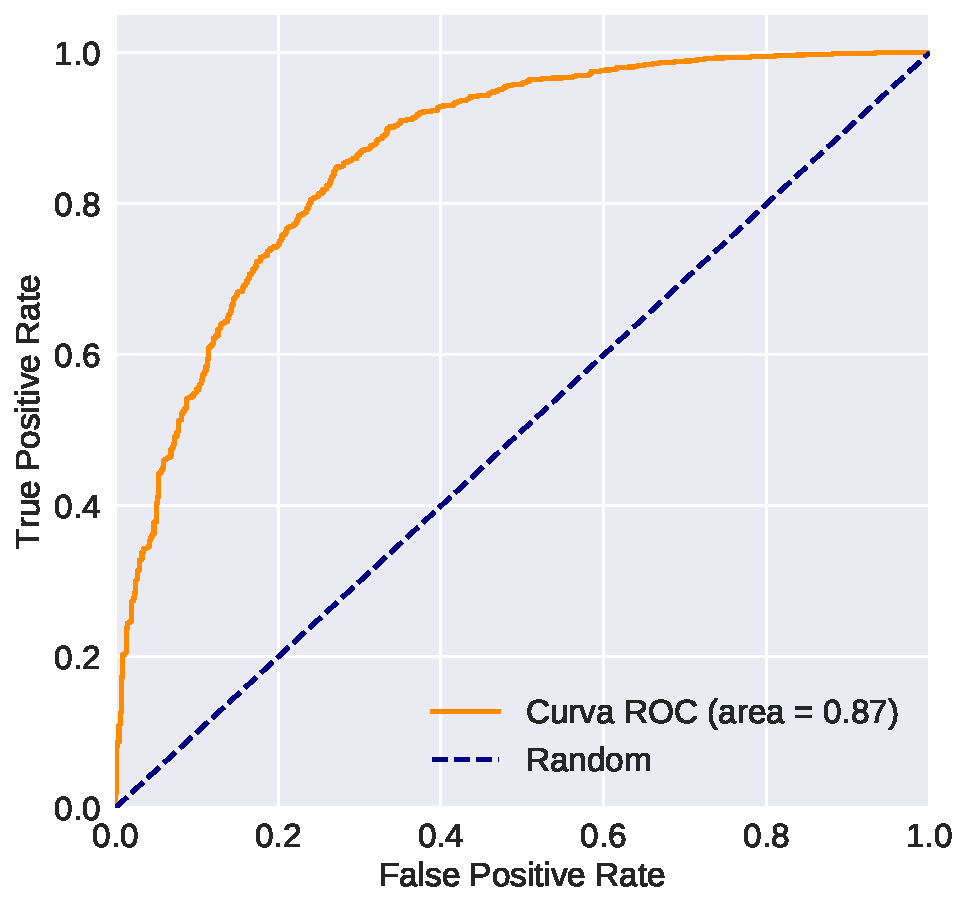
\includegraphics[width=\textwidth]{documents/latex/figures/3/integral_varq/auc_varq_integral.pdf}
    \caption{Curva AUC del algoritmo Random Forest del dataset Integral+VarQ Curado. La línea punteada corresponde a un predictor Random.}
    \label{fig:auc_integral_varq}
\end{subfigure}
\hfill
\hfill
\begin{subfigure}[b]{0.7\textwidth}
    \centering
    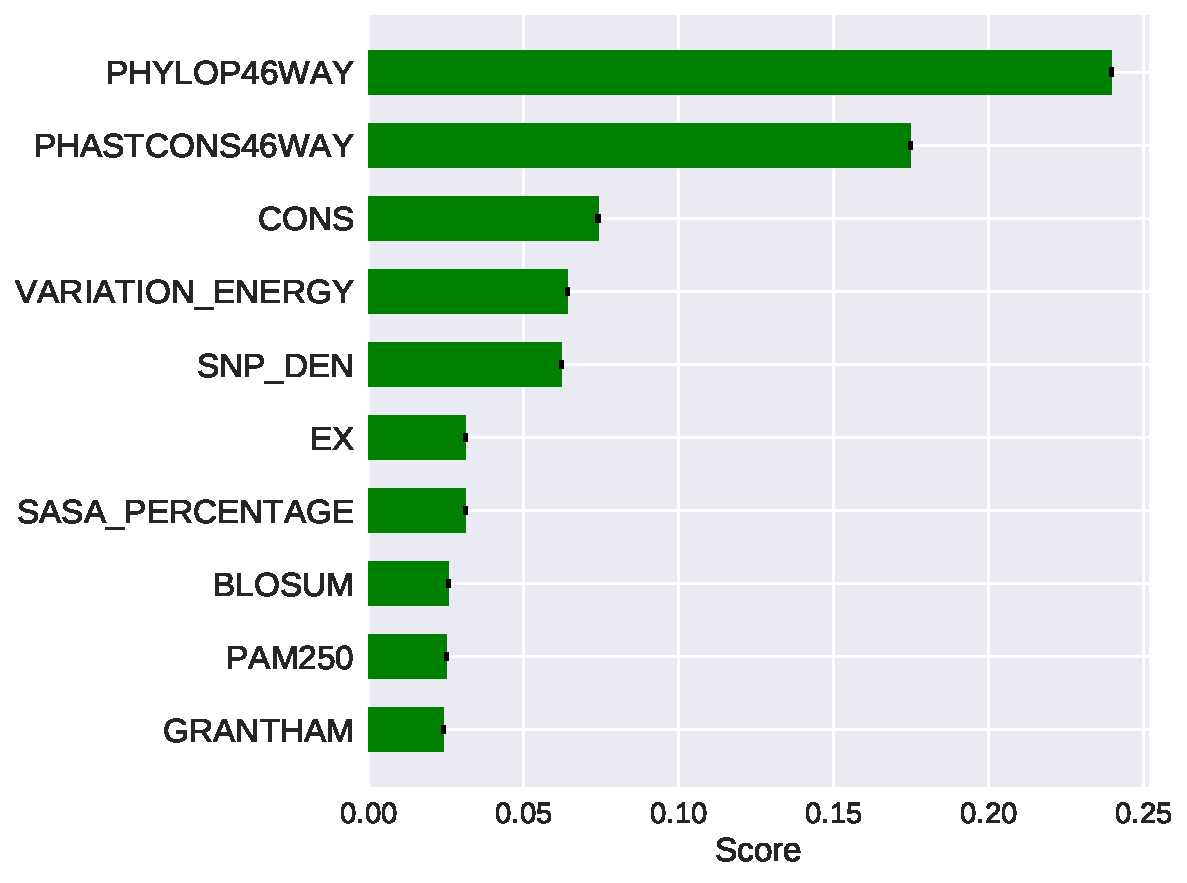
\includegraphics[width=\textwidth]{documents/latex/figures/3/integral_varq/importances_varq_integral.pdf}
    \caption{Los 10 atributos más importantes del dataset Integral+VarQ Curado.}
    \label{fig:importances_integral_varq}
\end{subfigure}
\end{figure}
